%==============================================================================
%  Assignment 4 : Design of a Common-Source Amplifier
%  Design and Analysis of Common Source Amplifiers -- SCL 180 nm CMOS
%
%  Compile:  latexmk -pdf main.tex      (or pdflatex x3)
%==============================================================================
\documentclass[12pt,a4paper]{article}

%------------------------------- packages ------------------------------------
\usepackage[T1]{fontenc}
\usepackage[utf8]{inputenc}
\usepackage{mathptmx}
\usepackage[margin=1in,headheight=15pt]{geometry}
\usepackage{amsmath,amssymb}
\usepackage{graphicx}
\usepackage{booktabs}
\usepackage{multirow}
\usepackage{array}
\usepackage{float}
\usepackage{placeins}
\usepackage[font=small,labelfont=bf]{caption}
\usepackage{subcaption}
\usepackage{enumitem}
\usepackage{xcolor}
\usepackage{fancyhdr}
\usepackage{microtype}
\usepackage{circuitikz}
\usepackage[hidelinks,bookmarks=true]{hyperref}

%------------------------------- styling -------------------------------------
\definecolor{hdrgrey}{gray}{0.35}
\definecolor{boxbg}{RGB}{242,246,250}
\definecolor{boxrule}{RGB}{90,130,170}
\definecolor{warnbg}{RGB}{255,249,232}
\definecolor{warnrule}{RGB}{200,150,40}

\pagestyle{fancy}
\fancyhf{}
\fancyhead[L]{\footnotesize\color{hdrgrey} Common Source Amplifiers -- SCL 180\,nm CMOS}
\fancyhead[R]{\footnotesize\color{hdrgrey} Mishka Singla (24116052)}
\fancyfoot[C]{\thepage}
\renewcommand{\headrulewidth}{0.4pt}

\setlength{\parskip}{4pt}
\renewcommand{\arraystretch}{1.22}
% inline math is dense in this report; give TeX extra room before it
% resorts to an overfull line
\setlength{\emergencystretch}{3em}
\newcolumntype{L}[1]{>{\raggedright\arraybackslash}p{#1}}

%------------------------------ unit macros ----------------------------------
% siunitx is not present in this TeX installation, so a minimal, consistent
% unit layer is defined here.  \U{} is used inside math mode throughout.
\newcommand{\U}[1]{\,\mathrm{#1}}
\newcommand{\dg}{^{\circ}}
\newcommand{\ohm}{\Omega}
\newcommand{\kohm}{\mathrm{k}\Omega}
\newcommand{\um}{\mu\mathrm{m}}
\newcommand{\uA}{\mu\mathrm{A}}
\newcommand{\uW}{\mu\mathrm{W}}
\newcommand{\uS}{\mu\mathrm{S}}
\newcommand{\WL}{\left(\dfrac{W}{L}\right)}
\newcommand{\WLi}[1]{\left(W/L\right)_{#1}}

% boxed remarks
\newenvironment{keybox}
  {\par\vspace{4pt}\noindent
   \begin{lrbox}{\keyboxreg}\begin{minipage}{0.945\textwidth}\small\vspace{2pt}}
  {\vspace{2pt}\end{minipage}\end{lrbox}%
   \fcolorbox{boxrule}{boxbg}{\usebox{\keyboxreg}}\par\vspace{4pt}}
\newsavebox{\keyboxreg}

\newcommand{\flag}[1]{%
  \par\vspace{4pt}\noindent
  \fcolorbox{warnrule}{warnbg}{%
    \begin{minipage}{0.955\textwidth}\small\vspace{2pt}#1\vspace{2pt}\end{minipage}}%
  \par\vspace{4pt}}

%==============================================================================
\begin{document}

%------------------------------- title page ----------------------------------
\begin{titlepage}
\centering
\vspace*{1.2cm}
{\large Course: TEB-102\par}
\vspace{2.4cm}
\rule{\textwidth}{1.2pt}\\[0.5cm]
{\LARGE\bfseries Assignment 4\\[0.35cm]
Design and Analysis of\\[0.15cm]
Common Source Amplifiers\par}
\vspace{0.45cm}
{\large Resistive, PMOS Active and PMOS Diode-Connected Loads\\
in SCL 180\,nm CMOS Technology\par}
\vspace{0.4cm}
\rule{\textwidth}{1.2pt}\\[1.6cm]

\begin{tabular}{rl}
\textbf{Name}            & Mishka Singla \\
\textbf{Enrollment No.}  & 24116052 \\
\textbf{Technology}      & SCL 180\,nm CMOS (\texttt{ts018\_scl\_prim}) \\
\textbf{Supply}          & $V_{DD} = 1.8\U{V}$ \\
\textbf{Load capacitor}  & $C_L = 50\U{fF}$ \\
\textbf{Tool}            & Cadence Virtuoso 6.1.7, Spectre simulator \\
\textbf{Simulation temp.}& $27\dg$C \\
\end{tabular}

\vfill
\vspace{1.0cm}
\end{titlepage}

\tableofcontents
\clearpage
\listoffigures
\listoftables
\clearpage

%==============================================================================
\section{Objective}
%==============================================================================
The objective of this experiment is to design, hand-analyse and simulate a
common-source (CS) CMOS voltage amplifier in SCL 180\,nm technology that
simultaneously satisfies a DC voltage gain of at least $15\U{dB}$, a power
dissipation not exceeding $1\U{mW}$, and a $-3\U{dB}$ bandwidth of at least
$100\U{MHz}$ while driving a $50\U{fF}$ load capacitor.

The amplifier is to be realised with three different load devices:

\begin{enumerate}[label=(\alph*),leftmargin=2.2em,itemsep=2pt]
  \item a \textbf{resistive load} (the required load resistance is to be determined),
  \item a \textbf{PMOS active load} (current-source load, gate biased from a
        separate reference), and
  \item a \textbf{PMOS diode-connected load}.
\end{enumerate}

For each topology the transistor dimensions $(W/L)$ are to be computed at the
minimum channel length $L_{\min} = 180\U{nm}$, a biasing network based on a
current mirror is to be designed to establish the quiescent drain current, the
region of operation of every transistor is to be reported, the small-signal
parameters ($R_{in}$, $R_{out}$, $g_m$, $A_{v0}$, $f_{-3\U{dB}}$) are to be
obtained analytically, and the design is to be verified by DC, AC and transient
simulation. Finally the three configurations are to be compared against one
another and against the hand calculations.

%==============================================================================
\section{Design Specifications}
%==============================================================================
The specifications extracted verbatim from the assignment statement are listed
in Table~\ref{tab:specs}. Every one of these is revisited in the compliance
audit of Section~\ref{sec:compliance}.

\begin{table}[H]
\centering
\caption{Design specifications imposed by the assignment.}
\label{tab:specs}
\begin{tabular}{llc}
\toprule
\textbf{Parameter} & \textbf{Requirement} & \textbf{Symbol} \\
\midrule
DC voltage gain          & $\geq 15\U{dB}$ ($\equiv 5.623\U{V/V}$) & $A_{v0}$ \\
Power dissipation        & $\leq 1\U{mW}$                          & $P_{DC}$ \\
Bandwidth                & $\geq 100\U{MHz}$ ($-3\U{dB}$ or unity-gain) & $f_{-3\U{dB}}$ \\
Load capacitance         & $= 50\U{fF}$                            & $C_L$ \\
Channel length           & $= 180\U{nm}$ (minimum, for speed)      & $L_{\min}$ \\
Supply voltage           & $1.8\U{V}$ (technology nominal)         & $V_{DD}$ \\
\bottomrule
\end{tabular}
\end{table}

The gain specification in linear terms is
\begin{equation}
|A_{v0}|_{\min} = 10^{15/20} = 10^{0.75} = 5.623\U{V/V}.
\label{eq:gainspec}
\end{equation}

The power specification sets a ceiling on the quiescent branch current:
\begin{equation}
I_D \leq \frac{P_{DC,\max}}{V_{DD}} = \frac{1\U{mW}}{1.8\U{V}} = 555.6\U{\mu A}.
\label{eq:idmax}
\end{equation}

%==============================================================================
\section{Theoretical Background}
%==============================================================================

\subsection{The common-source stage}
In a common-source amplifier the input signal is applied to the gate of an NMOS
transistor, the output is taken at the drain, and the source is tied to the AC
ground. A small increase in $v_{GS}$ increases the drain current, which pulls
the drain node \emph{down}; the stage is therefore \textbf{inverting}, which is
the defining signature verified later in the transient analysis
(Section~\ref{sec:tran}).

\subsection{Large-signal model}
With the transistor biased in saturation and using the square-law
approximation,
\begin{equation}
I_D = \tfrac{1}{2}\,\mu_n C_{ox}\WL_n V_{OV}^{2}\,(1+\lambda V_{DS}),
\qquad V_{OV} = V_{GS}-V_{TH}.
\label{eq:idsat}
\end{equation}
The saturation condition that must be checked for every device is
\begin{equation}
V_{DS} \;\geq\; V_{OV} \;=\; V_{GS}-V_{TH}
\qquad\text{(NMOS)},\qquad
|V_{DS}| \;\geq\; |V_{GS}|-|V_{TH}|
\quad\text{(PMOS)}.
\label{eq:satcond}
\end{equation}

\subsection{Small-signal parameters}
Differentiating \eqref{eq:idsat} gives the transconductance and the
channel-length-modulation output resistance:
\begin{equation}
g_m = \frac{2 I_D}{V_{OV}} = \sqrt{2\,\mu_n C_{ox}\WL_n I_D},
\qquad
r_o = \frac{1}{\lambda I_D}.
\label{eq:gmro}
\end{equation}
Equation~\eqref{eq:gmro} inverted gives the sizing relation used throughout
Section~\ref{sec:calc}:
\begin{equation}
\WL = \frac{g_m^{2}}{2\,\mu C_{ox} I_D}.
\label{eq:sizing}
\end{equation}

\subsection{Gain of the three load configurations}
All three stages share the same small-signal form
$A_{v0} = -g_{m,n} R_{out}$; only $R_{out}$ differs.

\begin{table}[H]
\centering
\caption{Output resistance and gain expression for each load type.}
\label{tab:loadexpr}
\begin{tabular}{llL{5.9cm}}
\toprule
\textbf{Load} & \textbf{$R_{out}$} & \textbf{Gain} \\
\midrule
Resistive $R_D$ & $R_D \parallel r_{o,n}$ &
  $A_{v0}=-g_{m,n}(R_D\parallel r_{o,n})\approx -g_{m,n}R_D$ \\
PMOS active     & $r_{o,n}\parallel r_{o,p}$ &
  $A_{v0}=-g_{m,n}(r_{o,n}\parallel r_{o,p})$ --- intrinsic gain, largest \\
PMOS diode      & $\dfrac{1}{g_{m,p}}\parallel r_{o,n}\parallel r_{o,p}$ &
  $A_{v0}\approx-\dfrac{g_{m,n}}{g_{m,p}}
   =-\sqrt{\dfrac{\mu_n C_{ox}\WLi{n}}{\mu_p C_{ox}\WLi{p}}}$ \\
\bottomrule
\end{tabular}
\end{table}

The diode-connected case is noteworthy: its gain reduces to a \emph{ratio of
device transconductances}, so it is set by the device dimensions and the
mobility ratio rather than by an external component. That gain is
intrinsically low, however, because the diode connection presents the small
effective resistance $1/g_{m,p}$ at the output node. In exchange, the load is
compact --- a single transistor, with no resistor and no external bias
reference, since the gate--drain short biases it itself.

\subsection{Frequency response}
Each stage is a single dominant-pole system whose pole is formed by the output
resistance and the total capacitance at the output node:
\begin{equation}
A_v(s) = \frac{-g_{m,n}R_{out}}{1+sR_{out}C_{tot}},
\qquad
f_{-3\U{dB}} = \frac{1}{2\pi R_{out} C_{tot}}.
\label{eq:f3db}
\end{equation}
Here $C_{tot}=C_L+C_{par}$, where $C_{par}$ lumps the drain-bulk junction
capacitances of both devices and the gate-drain overlap capacitance. The
gain--bandwidth product is accordingly
\begin{equation}
\mathrm{GBW} = |A_{v0}|\cdot f_{-3\U{dB}} = \frac{g_{m,n}}{2\pi C_{tot}},
\label{eq:gbw}
\end{equation}
which is independent of $R_{out}$: \emph{raising the load resistance trades
bandwidth for gain one-for-one}. This trade-off is the central experimental
observation of this assignment.

The corresponding phase, for an inverting single-pole stage, is
\begin{equation}
\angle A_v(f) = -180\dg - \arctan\!\left(\frac{f}{f_{-3\U{dB}}}\right),
\label{eq:phase}
\end{equation}
i.e.\ $-180\dg$ in mid-band (the inversion), $-225\dg$ exactly at
$f_{-3\U{dB}}$, and $-270\dg$ asymptotically.

\subsection{Input and output impedance}
The MOSFET gate is insulated, therefore at DC
\begin{equation}
R_{in} \to \infty .
\end{equation}
At signal frequencies the input is capacitive, and because the gate--drain
capacitance bridges an inverting gain it is multiplied by the Miller effect:
\begin{equation}
C_{in} = C_{gs} + (1+|A_{v0}|)\,C_{gd},
\qquad
Z_{in}(j\omega) = \frac{1}{j\omega C_{in}} .
\label{eq:cin}
\end{equation}
The output impedance is the $R_{out}$ of Table~\ref{tab:loadexpr} in parallel
with $C_{tot}$.

\subsection{Output swing}
The output voltage must keep the driving NMOS in saturation at the bottom of
the swing and the load device functional at the top:
\begin{align}
\text{resistive:}\quad & V_{OV,n} \leq v_{OUT} \leq V_{DD} \label{eq:swr}\\
\text{active load:}\quad & V_{OV,n} \leq v_{OUT} \leq V_{DD}-|V_{OV,p}| \label{eq:swa}\\
\text{diode load:}\quad & V_{OV,n} \leq v_{OUT} \leq V_{DD}-|V_{TH,p}| \label{eq:swd}
\end{align}
The maximum \emph{symmetric} peak-to-peak swing about a quiescent point
$V_{OUT,Q}$ is
\begin{equation}
V_{out,pp}^{\max} = 2\,\min\!\big(V_{OUT,Q}-v_{OUT,\min},\;
                                   v_{OUT,\max}-V_{OUT,Q}\big).
\label{eq:swing}
\end{equation}
Equation~\eqref{eq:swd} is the reason the diode-connected load is the weakest
of the three: its upper limit is set by a \emph{threshold} voltage rather than
an overdrive voltage, costing roughly $400\U{mV}$ of headroom.

\subsection{Power dissipation}
With a single branch carrying $I_D$ from a $V_{DD}$ rail,
\begin{equation}
P_{DC} = V_{DD}\,I_D .
\label{eq:power}
\end{equation}

%==============================================================================
\section{Design Methodology}
%==============================================================================
The design proceeds in the following order, which is the order in which the
assignment poses its questions:

\begin{enumerate}[leftmargin=2.0em,itemsep=2pt]
  \item Convert the gain and bandwidth specifications into a required
        $g_m$ and a permissible $R_{out}$ via \eqref{eq:f3db} and
        \eqref{eq:gbw}.
  \item Choose $I_D$ within the power budget \eqref{eq:idmax}, leaving margin.
  \item Choose an overdrive $V_{OV}$ --- small enough for good $g_m/I_D$
        efficiency, large enough to stay out of sub-threshold and to preserve
        output swing. Values in the $100$--$160\U{mV}$ range are used here.
  \item Compute $(W/L)$ from \eqref{eq:sizing} at $L = L_{\min} = 180\U{nm}$.
  \item Design the current-mirror reference branch that establishes $I_D$.
  \item Verify saturation for every device using \eqref{eq:satcond}.
  \item Simulate (DC, AC, transient) and compare.
\end{enumerate}

The process constants used for all hand calculations are collected in
Table~\ref{tab:proc}.

\begin{table}[H]
\centering
\caption{Process constants assumed for the SCL 180\,nm hand calculations.}
\label{tab:proc}
\begin{tabular}{llc}
\toprule
\textbf{Quantity} & \textbf{Symbol} & \textbf{Value} \\
\midrule
NMOS transconductance parameter & $\mu_n C_{ox}$ & $270\U{\mu A/V^2}$ \\
PMOS transconductance parameter & $\mu_p C_{ox}$ & $70\U{\mu A/V^2}$ \\
Channel-length modulation ($L=180\U{nm}$) & $\lambda_n=\lambda_p$ & $0.28\U{V^{-1}}$ \\
Gate oxide capacitance & $C_{ox}$ & $8.5\U{fF/\mu m^2}$ \\
Supply & $V_{DD}$ & $1.8\U{V}$ \\
Load capacitance & $C_L$ & $50\U{fF}$ \\
\bottomrule
\end{tabular}
\end{table}

\flag{\textbf{Assumption A1.} The SCL 180\,nm model card is proprietary and its
parameters are not printed by the schematic annotation. The values of
$\mu C_{ox}$, $\lambda$ and $C_{ox}$ in Table~\ref{tab:proc} are standard
published figures for a 180\,nm bulk CMOS process and are used \emph{only} for
the analytical column. Every ``simulation'' number in this report is read
directly from the Cadence annotations and is independent of this assumption.}

\subsection{Translating the specifications into circuit quantities}
From the gain requirement \eqref{eq:gainspec} and the bandwidth requirement,
combining into the gain--bandwidth product \eqref{eq:gbw} with
$C_{tot}\approx C_L = 50\U{fF}$:
\begin{equation}
g_{m,n} \;\geq\; 2\pi\,C_{tot}\cdot |A_{v0}|_{\min}\cdot f_{-3\U{dB},\min}
       = 2\pi(50\times10^{-15})(5.623)(100\times10^{6})
       = 176.7\U{\mu S}.
\end{equation}
This is a very relaxed requirement; the bias currents actually used
($244$--$340\U{\mu A}$) give $g_m$ values more than an order of magnitude
larger, so the real design constraint is \emph{not} the gain floor but the
simultaneous satisfaction of swing, saturation margin and power.

For the resistive-load case the bandwidth requirement caps the load resistor:
\begin{equation}
R_D \;\leq\; \frac{1}{2\pi C_L f_{-3\U{dB},\min}}
    = \frac{1}{2\pi (50\times10^{-15})(100\times10^{6})}
    = 31.83\U{k\Omega}.
\end{equation}
A much smaller $R_D=3\U{k\Omega}$ was ultimately chosen (Section~\ref{sec:calcres})
to place the quiescent output at mid-rail while keeping $I_D$ inside the power
budget --- the resulting bandwidth is then far in excess of the minimum.

%==============================================================================
\section{Chosen Hand-Calculation Design Point (Q2, Q3 and Q4)}\label{sec:handcalc}
%==============================================================================
The assignment fixes the \emph{performance targets} (Q1) but leaves the
designer free to choose the bias current, the overdrive voltage and the process
constants used for the paper design. This section answers Q2, Q3 and Q4
directly as a self-contained hand design at the design point chosen for the
hand calculation, so that each question has an explicit closed-form answer.
The values used are collected in Table~\ref{tab:handpoint}.
Section~\ref{sec:calc} then analyses the circuits that were actually built and
simulated in Cadence, which were biased differently.

\flag{\textbf{Two separate things, kept separate.} The numbers in this section
are a \emph{paper design}. They are \textbf{not} measurements, and they are not
the circuit that was simulated. Everything from Section~\ref{sec:cadence}
onwards reports the actual implemented circuits. Where the two differ --- and
they do --- the measured values govern. See
Section~\ref{sec:handvsimpl} for the side-by-side comparison, and
assumption~A9 in Appendix~\ref{app:assumptions}.}

\subsection{The chosen design point}
\begin{table}[H]
\centering
\caption{Values chosen for the hand calculations of Q2--Q4.}
\label{tab:handpoint}
\small
\begin{tabular}{llcl}
\toprule
\textbf{Quantity} & \textbf{Symbol} & \textbf{Value} & \textbf{Used in} \\
\midrule
Supply voltage                  & $V_{DD}$        & $1.8\U{V}$          & Q2, Q3, Q4 \\
Channel length                  & $L$             & $180\U{nm}$         & Q2, Q3 \\
Load capacitance                & $C_L$           & $50\U{fF}$          & Q4 \\
\addlinespace[2pt]
Drain current                   & $I_D$           & $500\U{\mu A}$      & Q2, Q3 \\
Overdrive voltage               & $V_{OV}$        & $0.25\U{V}$         & Q2, Q3 \\
NMOS process parameter          & $\mu_n C_{ox}$  & $200\U{\mu A/V^2}$  & Q2, Q3 \\
PMOS process parameter          & $\mu_p C_{ox}$  & $100\U{\mu A/V^2}$  & Q2, Q3 \\
Threshold voltage               & $|V_{TH}|$      & $0.5\U{V}$          & Q3 \\
\addlinespace[2pt]
Drain current                   & $I_D$           & $100\U{\mu A}$      & Q4 \\
Overdrive voltage               & $V_{OV}$        & $0.2\U{V}$          & Q4 \\
Channel-length modulation       & $\lambda$       & $0.05\U{V^{-1}}$    & Q4 \\
Drain resistor                  & $R_D$           & $18\U{k\Omega}$     & Q4 \\
\bottomrule
\end{tabular}
\end{table}

Note that Q4 is posed at a \emph{different} operating point ($100\U{\mu A}$,
$V_{OV}=0.2\U{V}$) from Q2 and Q3 ($500\U{\mu A}$, $V_{OV}=0.25\U{V}$). The two
are therefore treated as two separate chosen cases and are not mixed.

%------------------------------------------------------------------
\subsection{Q2 --- Transistor sizing at the chosen design point}
\label{sec:q2}
%------------------------------------------------------------------
The saturation drain-current expression \eqref{eq:idsat}, neglecting
channel-length modulation, is rearranged for the aspect ratio:
\begin{equation}
I_D = \tfrac{1}{2}\,\mu C_{ox}\WL V_{OV}^{2}
\qquad\Longrightarrow\qquad
\WL = \frac{2 I_D}{\mu C_{ox}\,V_{OV}^{2}} .
\label{eq:q2sizing}
\end{equation}

\paragraph{NMOS driver.}
Substituting $I_D = 500\U{\mu A}$, $\mu_n C_{ox} = 200\U{\mu A/V^2}$ and
$V_{OV} = 0.25\U{V}$ into \eqref{eq:q2sizing}:
\begin{align*}
\WLi{n} &= \frac{2\,(500\times10^{-6})}
                {(200\times10^{-6})(0.25)^{2}}
         = \frac{1\times10^{-3}}{(200\times10^{-6})(0.0625)}
         = \frac{1\times10^{-3}}{1.25\times10^{-5}}\\[2pt]
\WLi{n} &= \mathbf{80}
\qquad\Longrightarrow\qquad
W_n = 80 \times 0.18\U{\mu m} = 14.4\U{\mu m}.
\end{align*}

\paragraph{PMOS active load.}
The load device carries the same $500\U{\mu A}$ at the same overdrive, but with
$\mu_p C_{ox} = 100\U{\mu A/V^2}$:
\begin{align*}
\WLi{p} &= \frac{2\,(500\times10^{-6})}
                {(100\times10^{-6})(0.25)^{2}}
         = \frac{1\times10^{-3}}{6.25\times10^{-6}}\\[2pt]
\WLi{p} &= \mathbf{160}
\qquad\Longrightarrow\qquad
W_p = 160 \times 0.18\U{\mu m} = 28.8\U{\mu m}.
\end{align*}

\paragraph{Check.}
Because both devices carry the same current at the same overdrive, their
aspect ratios must be in inverse proportion to their mobilities:
\[
\frac{\WLi{p}}{\WLi{n}} = \frac{160}{80} = 2
= \frac{\mu_n C_{ox}}{\mu_p C_{ox}} = \frac{200}{100} = 2 .\;\checkmark
\]
The resulting transconductance and power are
\begin{align*}
g_m    &= \frac{2 I_D}{V_{OV}} = \frac{2(500\times10^{-6})}{0.25} = 4\U{mS},\\
P_{DC} &= V_{DD} I_D = (1.8)(500\times10^{-6}) = 900\U{\mu W}
          \;\leq\; 1\U{mW}.\;\checkmark
\end{align*}
The power figure consumes $90\%$ of the budget, which becomes the binding
constraint on the bias network designed next.

\begin{table}[H]
\centering
\caption{Q2 result --- transistor dimensions at the chosen design point.}
\label{tab:q2}
\begin{tabular}{lccc}
\toprule
\textbf{Device} & $(W/L)$ & $L$ & $W$ \\
\midrule
NMOS driver $M_0$      & $80$  & $180\U{nm}$ & $14.4\U{\mu m}$ \\
PMOS active load $M_1$ & $160$ & $180\U{nm}$ & $28.8\U{\mu m}$ \\
\bottomrule
\end{tabular}
\end{table}

%------------------------------------------------------------------
\subsection{Q3 --- Current-mirror bias design for $I_D = 500\U{\mu A}$}
\label{sec:q3}
%------------------------------------------------------------------
Q3 asks for a biasing circuit --- a current source built from a current mirror
--- that establishes the quiescent drain current, and for the region of
operation of each transistor. The topology is the one drawn in
Figure~\ref{fig:mirror}.

\paragraph{Mirror relationship.}
For two devices sharing a gate--source voltage and both in saturation, the
currents scale with the aspect ratios:
\begin{equation}
\frac{I_{OUT}}{I_{REF}} = \frac{\WLi{out}}{\WLi{ref}} \;\equiv\; N .
\label{eq:mirror}
\end{equation}

\paragraph{Choosing the reference current from the power budget.}
A unity-ratio mirror ($N=1$) would require $I_{REF}=500\U{\mu A}$, so the
reference branch alone would double the supply current to $1\U{mA}$ and the
total dissipation to $1.8\U{mW}$ --- violating the $1\U{mW}$ specification.
The reference current must therefore be \emph{scaled down}. The budget allows
\[
I_{REF} \;\leq\; \frac{P_{DC,\max}}{V_{DD}} - I_D
        = \frac{1\U{mW}}{1.8\U{V}} - 500\U{\mu A}
        = 555.6 - 500 = 55.6\U{\mu A}.
\]
Choosing the round value $I_{REF} = 50\U{\mu A}$ gives the mirror ratio
\[
N = \frac{I_{OUT}}{I_{REF}} = \frac{500\U{\mu A}}{50\U{\mu A}} = 10 .
\]

\paragraph{Sizing the reference device.}
From \eqref{eq:mirror} with $\WLi{out} = 80$ (the Q2 result),
\[
\WLi{ref} = \frac{\WLi{out}}{N} = \frac{80}{10} = 8
\qquad\Longrightarrow\qquad
W_{ref} = 8 \times 0.18\U{\mu m} = 1.44\U{\mu m}.
\]
Verifying that this device really does sit at the same overdrive, which is
what makes the mirror accurate:
\[
I_{REF} = \tfrac{1}{2}(200\times10^{-6})(8)\,V_{OV}^{2}
        = (800\times10^{-6})V_{OV}^{2} = 50\times10^{-6},
\]
\[
\Rightarrow\quad V_{OV}^{2} = 0.0625
\quad\Rightarrow\quad
V_{OV} = 0.25\U{V}.\;\checkmark
\]
Both devices therefore share $V_{GS} = V_{TH}+V_{OV} = 0.5+0.25 = 0.75\U{V}$.

\paragraph{Reference resistor.}
The resistor drops the remainder of the supply across the reference branch:
\[
R_{REF} = \frac{V_{DD}-V_{GS}}{I_{REF}}
        = \frac{1.8 - 0.75}{50\times10^{-6}}
        = \frac{1.05}{50\times10^{-6}}
        = \mathbf{21\U{k\Omega}}.
\]

\paragraph{Output current.}
\[
I_{OUT} = N\,I_{REF} = 10 \times 50\U{\mu A} = \mathbf{500\U{\mu A}}.\;\checkmark
\]

\paragraph{PMOS side (for the active-load configuration).}
The same reference branch biases a PMOS mirror whose output device is the
$\WLi{p}=160$ load of Q2. Scaling by the same $N = 10$,
\[
\WLi{p,ref} = \frac{160}{10} = 16,
\qquad
I_{REF} = \tfrac{1}{2}(100\times10^{-6})(16)(0.25)^{2} = 50\U{\mu A},\;\checkmark
\]
so the PMOS reference also sits at $|V_{OV}| = 0.25\U{V}$, i.e.\
$|V_{GS}| = 0.75\U{V}$, and its reference resistor is likewise $21\U{k\Omega}$.
Because the driver and the active load are in series in the same branch, they
share the single $500\U{\mu A}$ current, so only one reference branch is
needed.

\paragraph{Total power check.}
\[
P_{DC,\text{total}} = V_{DD}\,(I_D + I_{REF})
 = 1.8\,(500+50)\times10^{-6} = 990\U{\mu W} \;\leq\; 1\U{mW}.\;\checkmark
\]

\paragraph{Region of operation.}
Every transistor in the bias network and the amplifier must satisfy
\eqref{eq:satcond}, i.e.\ $|V_{DS}| \geq |V_{OV}| = 0.25\U{V}$:

\begin{table}[H]
\centering
\caption{Q3 result --- bias design and region of operation at the chosen
design point.}
\label{tab:q3}
\small
\begin{tabular}{llrrl}
\toprule
\textbf{Device} & \textbf{Role} & $(W/L)$ & \textbf{Current} & \textbf{Region} \\
\midrule
$M_{ref,n}$ & NMOS reference (diode-connected) & $8$   & $50\U{\mu A}$  & Saturation (by connection) \\
$M_0$       & NMOS driver (mirror output)      & $80$  & $500\U{\mu A}$ & Saturation ($V_{DS}=0.9 > 0.25$) \\
$M_{ref,p}$ & PMOS reference (diode-connected) & $16$  & $50\U{\mu A}$  & Saturation (by connection) \\
$M_1$       & PMOS active load (mirror output) & $160$ & $500\U{\mu A}$ & Saturation ($|V_{DS}|=0.9 > 0.25$) \\
\midrule
\multicolumn{3}{l}{Reference resistor $R_{REF}$} & \multicolumn{2}{l}{$21\U{k\Omega}$} \\
\multicolumn{3}{l}{Mirror ratio $N$} & \multicolumn{2}{l}{$10$} \\
\multicolumn{3}{l}{Total dissipation} & \multicolumn{2}{l}{$990\U{\mu W}$} \\
\bottomrule
\end{tabular}
\end{table}

With the output node at mid-rail ($V_{OUT}=0.9\U{V}$), both amplifier devices
have $|V_{DS}| = 0.9\U{V}$, far above the $0.25\U{V}$ needed, so both are
comfortably saturated. The two diode-connected reference devices are saturated
by construction, since $V_{DS}=V_{GS}$ guarantees $|V_{DS}| > |V_{OV}|$.

%------------------------------------------------------------------
\subsection{Q4 --- Small-signal hand calculation at the chosen
            operating point}\label{sec:q4}
%------------------------------------------------------------------
Q4 asks for the input impedance, the output impedance, the DC gain and the
$-3\U{dB}$ frequency, calculated theoretically. The chosen case is
$I_D = 100\U{\mu A}$, $V_{OV} = 0.2\U{V}$, $\lambda = 0.05\U{V^{-1}}$ and a
resistive load $R_D = 18\U{k\Omega}$, driving the specified $C_L = 50\U{fF}$.

\paragraph{(a) Transconductance.}
\[
g_m = \frac{2 I_D}{V_{OV}}
    = \frac{2\,(100\times10^{-6})}{0.2}
    = \frac{200\times10^{-6}}{0.2}
    = \mathbf{1.000\U{mS}}.
\]

\paragraph{(b) Transistor output resistance.}
\[
r_o = \frac{1}{\lambda I_D}
    = \frac{1}{(0.05)(100\times10^{-6})}
    = \frac{1}{5\times10^{-6}}
    = \mathbf{200\U{k\Omega}}.
\]

\paragraph{(c) Input impedance.}
The gate is insulated from the channel by the oxide, so no DC current flows
into it:
\[
R_{in} = \mathbf{\infty} \quad\text{(at DC)} .
\]
At signal frequencies the input is purely capacitive, given by \eqref{eq:cin}:
\[
Z_{in}(j\omega) = \frac{1}{j\omega C_{in}},
\qquad
C_{in} = C_{gs} + (1+|A_{v0}|)C_{gd}
       = C_{gs} + 17.51\,C_{gd},
\]
using the gain computed in step (e) below.

\paragraph{(d) Output impedance.}
The drain resistor appears in parallel with the transistor output resistance:
\begin{align*}
R_{out} &= R_D \parallel r_o
         = \frac{R_D\,r_o}{R_D + r_o}
         = \frac{(18\times10^{3})(200\times10^{3})}{18\times10^{3}+200\times10^{3}}\\[2pt]
        &= \frac{3.6\times10^{9}}{218\times10^{3}}
         = \mathbf{16.514\U{k\Omega}} .
\end{align*}
Note that $R_D \ll r_o$, so the $18\U{k\Omega}$ resistor dominates and
$R_{out}$ lands only $8.3\%$ below $R_D$.

\paragraph{(e) DC voltage gain.}
\[
A_{v0} = -g_m\,R_{out}
       = -(1.000\times10^{-3})(16.514\times10^{3})
       = \mathbf{-16.514\U{V/V}},
\]
\[
|A_{v0}|_{\U{dB}} = 20\log_{10}(16.514) = \mathbf{24.36\U{dB}}
\;\geq\; 15\U{dB}.\;\checkmark
\]

\paragraph{(f) $-3\U{dB}$ frequency.}
The dominant pole is formed by $R_{out}$ and the load capacitance,
from \eqref{eq:f3db}:
\begin{align*}
f_{-3\U{dB}} &= \frac{1}{2\pi R_{out} C_L}
              = \frac{1}{2\pi (16.514\times10^{3})(50\times10^{-15})}
              = \frac{1}{5.1879\times10^{-9}}\\[2pt]
             &= \mathbf{192.75\U{MHz}} \;\geq\; 100\U{MHz}.\;\checkmark
\end{align*}

\paragraph{(g) Unity-gain frequency.}
From \eqref{eq:gbw},
\[
f_{u} = |A_{v0}|\,f_{-3\U{dB}} = \frac{g_m}{2\pi C_L}
      = \frac{1.000\times10^{-3}}{2\pi(50\times10^{-15})}
      = \mathbf{3.183\U{GHz}} .
\]

\paragraph{(h) Power dissipation.}
\[
P_{DC} = V_{DD} I_D = (1.8)(100\times10^{-6}) = \mathbf{180\U{\mu W}}
\;\leq\; 1\U{mW}.\;\checkmark
\]

\begin{table}[H]
\centering
\caption{Q4 result --- small-signal parameters at the chosen operating
point, and compliance with the Q1 specifications.}
\label{tab:q4}
\small
\begin{tabular}{llcl}
\toprule
\textbf{Parameter} & \textbf{Symbol} & \textbf{Value} & \textbf{Specification} \\
\midrule
Transconductance      & $g_m$             & $1.000\U{mS}$     & --- \\
Output resistance (device) & $r_o$        & $200\U{k\Omega}$  & --- \\
Input impedance       & $R_{in}$          & $\infty$ (DC)     & --- \\
Output impedance      & $R_{out}$         & $16.514\U{k\Omega}$ & --- \\
DC voltage gain       & $A_{v0}$          & $-16.514\U{V/V}$  & --- \\
DC voltage gain       & $|A_{v0}|_{\U{dB}}$ & $24.36\U{dB}$   & $\geq 15\U{dB}$ \checkmark \\
$-3\U{dB}$ frequency  & $f_{-3\U{dB}}$    & $192.75\U{MHz}$   & $\geq 100\U{MHz}$ \checkmark \\
Unity-gain frequency  & $f_u$             & $3.183\U{GHz}$    & --- \\
Power dissipation     & $P_{DC}$          & $180\U{\mu W}$    & $\leq 1\U{mW}$ \checkmark \\
\bottomrule
\end{tabular}
\end{table}

All three Q1 specifications are satisfied at this operating point.

%------------------------------------------------------------------
\subsection{Relationship between the hand design and the implemented
            circuits}\label{sec:handvsimpl}
%------------------------------------------------------------------
The circuits actually built in Cadence were biased at lower currents and
smaller overdrives than the hand-calculation design point, so their device
sizes and small-signal parameters differ. Table~\ref{tab:handvsimpl} makes the
difference explicit so that the two sets of numbers are never confused.

\begin{table}[H]
\centering
\caption{Hand-calculation design point versus the circuits actually
implemented and measured in Cadence.}
\label{tab:handvsimpl}
\footnotesize
\begin{tabular}{lcccc}
\toprule
& \multicolumn{1}{c}{\textbf{Hand design}} & \multicolumn{3}{c}{\textbf{Implemented (measured)}} \\
\cmidrule(lr){2-2}\cmidrule(lr){3-5}
\textbf{Quantity} & \textbf{Q2/Q3 (Q4)} & \textbf{A: Resistive} & \textbf{B: Active} & \textbf{C: Diode} \\
\midrule
$I_D$            & $500\U{\mu A}$ ($100$) & $303.01\U{\mu A}$ & $243.887\U{\mu A}$ & $340.35\U{\mu A}$ \\
$V_{OV,n}$       & $250\U{mV}$ ($200$)    & $152.988\U{mV}$   & $152.591\U{mV}$    & $107.496\U{mV}$ \\
$(W/L)_n$        & $80$                   & $51.8$            & $41.9$             & $85.6$ \\
$(W/L)_p$        & $160$                  & ---               & $212.2$            & $3.76$ \\
$g_{m,n}$        & $4\U{mS}$ ($1.000$)    & $2.91169\U{mS}$   & $2.34981\U{mS}$    & $3.96611\U{mS}$ \\
$R_D$            & ($18\U{k\Omega}$)      & $3.000\U{k\Omega}$& ---                & --- \\
$R_{out}$        & ($16.514\U{k\Omega}$)  & $2454.9\U{\Omega}$& $7234.6\U{\Omega}$ & $922.8\U{\Omega}$ \\
$|A_{v0}|$       & ($16.514$, $24.36\U{dB}$) & $7.1469$ ($17.09\U{dB}$) & $17.0$ ($24.61\U{dB}$) & $3.66$ ($11.27\U{dB}$) \\
$f_{-3\U{dB}}$   & ($192.75\U{MHz}$)      & $1.03276\U{GHz}$  & $218.483\U{MHz}$   & $1.89606\U{GHz}$ \\
$P_{DC}$         & $900\U{\mu W}$ ($180$) & $545.42\U{\mu W}$ & $438.99\U{\mu W}$  & $612.63\U{\mu W}$ \\
\bottomrule
\end{tabular}
\end{table}

Three observations follow from Table~\ref{tab:handvsimpl}.

\begin{enumerate}[leftmargin=2.0em,itemsep=2pt]
\item The hand design and the implemented designs are \emph{both} valid
      solutions to the Q1 specification --- they simply sit at different points
      on the same gain--bandwidth trade-off. The hand design trades bandwidth
      ($192.75\U{MHz}$) for gain ($24.36\U{dB}$) by using a large
      $18\U{k\Omega}$ load; the implemented resistive design does the reverse,
      using $3\U{k\Omega}$ to reach $1.03\U{GHz}$ at $17.09\U{dB}$.
\item The measured $(W/L)$ values of the implemented circuits
      (Section~\ref{sec:calc}) are \emph{back-calculated from the annotated}
      $g_m$ \emph{and} $I_D$, whereas the Q2 values are \emph{forward-designed}
      from a chosen $I_D$ and $V_{OV}$. They answer different questions and are
      not expected to agree.
\item The implemented circuits use ideal voltage sources for gate biasing
      rather than the current mirror designed in Section~\ref{sec:q3}; this is
      recorded as assumption~A2 and discussed in Section~\ref{sec:biasimpl}.
\end{enumerate}

%==============================================================================
\section{Design Calculations for the Implemented Circuits}\label{sec:calc}
%==============================================================================
This section analyses the three circuits that were actually built and simulated
in Cadence, using their measured operating points. It is distinct from the
paper design of Section~\ref{sec:handcalc}.

Every calculation below follows the pattern
\textbf{formula $\rightarrow$ substitution $\rightarrow$ result}.
The three configurations are kept strictly separate; no quantity belonging to
one topology is reused in another.

%------------------------------------------------------------------
\subsection{Configuration A --- Resistive load}\label{sec:calcres}
%------------------------------------------------------------------
\paragraph{Choice of bias current.}
Targeting roughly half the power budget, and applying \eqref{eq:power},
\[
I_{D,\text{target}} = 300\U{\mu A}
\quad\Rightarrow\quad
P_{DC} = V_{DD}I_D = (1.8)(300\times10^{-6}) = 540\U{\mu W} \;<\; 1\U{mW}.\;\checkmark
\]

\paragraph{Choice of load resistor.}
Placing the quiescent drain node near mid-rail, the drop across $R_D$ should be
about $V_{DD}/2 = 0.9\U{V}$:
\[
R_D = \frac{V_{DD}-V_{OUT,Q}}{I_D} = \frac{1.8-0.9}{300\times10^{-6}}
    = 3.00\U{k\Omega}.
\]
A $3.0\U{k\Omega}$ resistor is therefore instantiated. This is comfortably
below the $31.83\U{k\Omega}$ bandwidth ceiling.

\paragraph{Overdrive and transconductance.}
The simulated operating point gives $V_{GS}=630\U{mV}$ and
$V_{TH}=477.012\U{mV}$, hence
\[
V_{OV,n} = V_{GS}-V_{TH} = 630 - 477.012 = 152.988\U{mV},
\]
\[
g_{m,n}^{\text{(sq-law)}} = \frac{2I_D}{V_{OV}}
 = \frac{2(303.01\times10^{-6})}{0.152988} = 3.9614\U{mS}.
\]

\paragraph{Transistor sizing.}
From \eqref{eq:sizing}, using the simulated $g_m = 2.91169\U{mS}$ and
$I_D=303.01\U{\mu A}$:
\[
\WL_n = \frac{g_m^{2}}{2\,\mu_n C_{ox} I_D}
      = \frac{(2.91169\times10^{-3})^{2}}
             {2(270\times10^{-6})(303.01\times10^{-6})}
      = \frac{8.4780\times10^{-6}}{1.6363\times10^{-7}} = 51.8 .
\]
At $L = 180\U{nm}$ this gives
\[
W_n = 51.8 \times 0.18\U{\mu m} = 9.33\U{\mu m}.
\]

\paragraph{Output resistance and gain.}
\[
r_{o,n} = \frac{1}{\lambda I_D} = \frac{1}{(0.28)(303.01\times10^{-6})}
        = 11.787\U{k\Omega},
\]
\[
R_{out} = R_D \parallel r_{o,n}
        = \frac{(3000)(11787)}{3000+11787} = 2391.4\U{\Omega},
\]
\[
|A_{v0}| = g_m R_{out} = (3.9614\times10^{-3})(2391.4) = 9.473\U{V/V}
         \;\equiv\; 20\log_{10}(9.473) = 19.53\U{dB}.
\]

\paragraph{Bandwidth.}
\[
f_{-3\U{dB}} = \frac{1}{2\pi R_{out}C_L}
             = \frac{1}{2\pi(2391.4)(50\times10^{-15})} = 1.331\U{GHz}.
\]

\paragraph{Output swing.}
From \eqref{eq:swr} and \eqref{eq:swing}, the output is bounded by
$v_{OUT}\in[152.988\U{mV},\,1.8\U{V}]$, and the quiescent point is
$V_{OUT,Q}=890.971\U{mV}$:
\begin{align*}
V_{out,pp}^{\max} &= 2\min(890.971-152.988,\;1800-890.971)\\
                  &= 2(737.98) = 1.476\U{V}.
\end{align*}

\paragraph{Input capacitance.}
$C_{gs}\approx \tfrac{2}{3}W L C_{ox}
 = \tfrac{2}{3}(9.33)(0.18)(8.5\U{fF/\mu m^2}) = 9.52\U{fF}$, so with
$R_{in}|_{DC}\to\infty$ the input presents roughly
$C_{in}\approx 9.5\U{fF}+(1+7.15)C_{gd}$ by \eqref{eq:cin}.

%------------------------------------------------------------------
\subsection{Configuration B --- PMOS active load}
%------------------------------------------------------------------
\paragraph{Bias current and power.}
\[
I_{D,\text{target}} = 250\U{\mu A}
\quad\Rightarrow\quad
P_{DC} = (1.8)(250\times10^{-6}) = 450\U{\mu W} < 1\U{mW}.\;\checkmark
\]

\paragraph{Overdrives.}
From the annotated operating point ($I_D = 243.887\U{\mu A}$):
\[
V_{OV,n} = 630 - 477.409 = 152.591\U{mV},
\qquad
|V_{OV,p}| = 635 - 513.421 = 121.579\U{mV}.
\]

\paragraph{Transistor sizing.}
NMOS driver, using $g_{m,n}=2.34981\U{mS}$:
\begin{align*}
\WLi{n} &= \frac{(2.34981\times10^{-3})^{2}}
                {2(270\times10^{-6})(243.887\times10^{-6})}
         = \frac{5.5216\times10^{-6}}{1.3170\times10^{-7}} = 41.9\\
\Rightarrow\quad W_n &= 41.9\times 0.18\U{\mu m} = 7.55\U{\mu m}.
\end{align*}
PMOS active load, using $g_{m,p}=2.69169\U{mS}$ and
$\mu_p C_{ox}=70\U{\mu A/V^2}$:
\begin{align*}
\WLi{p} &= \frac{(2.69169\times10^{-3})^{2}}
                {2(70\times10^{-6})(243.887\times10^{-6})}
         = \frac{7.2452\times10^{-6}}{3.4144\times10^{-8}} = 212.2\\
\Rightarrow\quad W_p &= 212.2\times 0.18\U{\mu m} = 38.19\U{\mu m}.
\end{align*}
The PMOS is roughly $5\times$ wider than the NMOS, which is the expected
consequence of $\mu_p \approx \mu_n/4$ together with the smaller PMOS
overdrive.

\paragraph{Small-signal transconductance (square law).}
\[
g_{m,n}^{\text{(sq-law)}} = \frac{2(243.887\times10^{-6})}{0.152591}
                          = 3.1966\U{mS}.
\]

\paragraph{Output resistance and gain.}
\[
r_{o,n}=r_{o,p}=\frac{1}{\lambda I_D}
 =\frac{1}{(0.28)(243.887\times10^{-6})} = 14.643\U{k\Omega},
\]
\[
R_{out}=r_{o,n}\parallel r_{o,p} = \frac{14.643}{2} = 7.3215\U{k\Omega},
\]
\[
|A_{v0}| = (3.1966\times10^{-3})(7321.5) = 23.40\U{V/V} \equiv 27.39\U{dB}.
\]

\paragraph{Bandwidth.}
\[
f_{-3\U{dB}} = \frac{1}{2\pi(7321.5)(50\times10^{-15})} = 434.7\U{MHz}.
\]

\paragraph{Output swing.}
From \eqref{eq:swa}, $v_{OUT}\in[152.591\U{mV},\,1.8-0.121579=1.6784\U{V}]$,
with $V_{OUT,Q}=904.82\U{mV}$:
\[
V_{out,pp}^{\max} = 2\min(904.82-152.591,\;1678.42-904.82)
                  = 2(752.23) = 1.504\U{V}.
\]
This is the largest usable swing of the three topologies, because both limits
are set by \emph{overdrive} voltages.

%------------------------------------------------------------------
\subsection{Configuration C --- PMOS diode-connected load}
%------------------------------------------------------------------
\paragraph{Bias current and power.}
\[
I_{D,\text{target}} = 350\U{\mu A}
\quad\Rightarrow\quad
P_{DC} = (1.8)(350\times10^{-6}) = 630\U{\mu W} < 1\U{mW}.\;\checkmark
\]

\paragraph{Overdrives.}
With $I_D = 340.35\U{\mu A}$ from the annotation:
\[
V_{OV,n} = 590 - 482.504 = 107.496\U{mV},
\]
\[
|V_{OV,p}| = |V_{GS,p}|-|V_{TH,p}| = 1.66011 - 0.494997 = 1.1651\U{V}.
\]
The diode connection forces $V_{DS,p}=V_{GS,p}$, so the PMOS absorbs
$1.660\U{V}$ of the $1.8\U{V}$ rail and leaves only $139.89\U{mV}$ for the
NMOS drain. This is the root cause of every shortfall discussed later.

\paragraph{Transistor sizing.}
\[
\WLi{n} = \frac{(3.96611\times10^{-3})^{2}}
               {2(270\times10^{-6})(340.35\times10^{-6})}
        = \frac{1.5730\times10^{-5}}{1.8379\times10^{-7}} = 85.6
\;\Rightarrow\; W_n = 15.41\U{\mu m},
\]
\[
\WLi{p} = \frac{(423.063\times10^{-6})^{2}}
               {2(70\times10^{-6})(340.35\times10^{-6})}
        = \frac{1.7898\times10^{-7}}{4.7649\times10^{-8}} = 3.76
\;\Rightarrow\; W_p = 0.68\U{\mu m}.
\]

\paragraph{Consistency check on the geometry.}
The diode-load gain should equal the square root of the ratio of the
$\mu C_{ox}(W/L)$ products:
\[
\sqrt{\frac{\mu_n C_{ox}\WLi{n}}{\mu_p C_{ox}\WLi{p}}}
= \sqrt{\frac{(270)(85.6)}{(70)(3.76)}}
= \sqrt{\frac{23112}{263.2}} = \sqrt{87.8} = 9.37,
\]
which reproduces exactly the simulated ratio
$g_{m,n}/g_{m,p} = 3.96611\U{mS}/423.063\U{\mu S} = 9.37$.
The extracted dimensions are therefore internally consistent.

\paragraph{Small-signal transconductances (square law).}
\[
g_{m,n}^{\text{(sq-law)}} = \frac{2(340.35\times10^{-6})}{0.107496} = 6.3323\U{mS},
\qquad
g_{m,p}^{\text{(sq-law)}} = \frac{2(340.35\times10^{-6})}{1.1651} = 584.2\U{\mu S}.
\]
\[
\frac{1}{g_{m,p}} = \frac{1}{584.2\times10^{-6}} = 1711.7\U{\Omega}.
\]

\paragraph{Output resistance and gain.}
\[
r_{o,n}=r_{o,p}=\frac{1}{(0.28)(340.35\times10^{-6})} = 10.492\U{k\Omega},
\]
\[
R_{out} = \frac{1}{g_{m,p}} \parallel r_{o,n} \parallel r_{o,p}
        = 1711.7 \parallel 5246.2 = 1290.5\U{\Omega},
\]
\[
|A_{v0}| = (6.3323\times10^{-3})(1290.5) = 8.172\U{V/V} \equiv 18.25\U{dB}.
\]
The simplified ratio form of Table~\ref{tab:loadexpr} gives
$|A_{v0}|\approx g_{m,n}/g_{m,p} = 10.84$, the difference being the loading of
$r_{o,n}\parallel r_{o,p}$.

\paragraph{Bandwidth.}
\[
f_{-3\U{dB}} = \frac{1}{2\pi(1290.5)(50\times10^{-15})} = 2.467\U{GHz}.
\]

\paragraph{Output swing.}
From \eqref{eq:swd}, $v_{OUT}\in[107.496\U{mV},\;1.8-0.494997=1.305\U{V}]$.
With the actual quiescent point $V_{OUT,Q} = 139.89\U{mV}$:
\[
V_{out,pp}^{\max} = 2\min(139.89-107.496,\;1305.0-139.89)
                  = 2(32.394) = 64.8\U{mV}.
\]
\begin{keybox}
\textbf{Critical finding.} The quiescent output of the diode-connected stage
sits only $32.4\U{mV}$ above the triode boundary. The stage is biased at the
very edge of saturation, which simultaneously destroys the output swing and
collapses $r_{o,n}$ --- and therefore the gain. This single fact explains the
entire shortfall discussed in Section~\ref{sec:tvs}.
\end{keybox}

%==============================================================================
\section{Biasing Circuit Design for the Implemented Circuits}
\label{sec:biasimpl}
%==============================================================================
Section~\ref{sec:q3} answered Q3 at the chosen hand-calculation design point
($I_D = 500\U{\mu A}$, mirror ratio $N=10$, $R_{REF}=21\U{k\Omega}$). This
section applies the same method to the \emph{as-implemented} operating points,
so that the bias network matches the circuits that were actually simulated, and
reports the region of operation of every transistor in them.

\subsection{Current-mirror reference branches}
In each case a reference branch sets $I_{REF}$ with a resistor, and a matched
device mirrors it into the amplifier. Sizing the reference device identically
to the mirrored device gives a $1\!:\!1$ ratio,
$I_D = I_{REF}\,(W/L)_{\text{out}}/(W/L)_{\text{ref}}$.

\begin{figure}[H]
\centering
\begin{circuitikz}[american, scale=0.80, transform shape]
% ---------------- (a) NMOS mirror ----------------
\begin{scope}
  \draw (0,3.6) node[vcc]{$V_{DD}$} -- (0,3.0);
  \draw (0,3.0) to[R, l=$R_{REF}$] (0,1.4);
  \draw (0,0) node[nmos, xscale=-1](Mr){};
  \draw (Mr.drain) -- (0,1.4);
  \draw (Mr.source) -- (0,-1.3) node[ground]{};
  \draw (Mr.gate) -- (0.9,0);
  \draw (0.9,0) node[circ]{} -- (0.9,1.4) -- (0,1.4);
  \draw (3.6,0) node[nmos](Mo){};
  \draw (Mo.source) -- (3.6,-1.3) node[ground]{};
  \draw (Mo.drain) -- (3.6,2.0) node[above, font=\footnotesize]{to $R_D$ / load};
  \draw (0.9,0) -- (Mo.gate);
  \node[font=\footnotesize] at (-1.0,0.75) {$M_{ref}$};
  \node[font=\footnotesize] at (4.6,0.75) {$M_{0}$};
  \node[font=\footnotesize, align=center] at (1.8,-2.9)
       {(a) NMOS mirror --- sets $I_D$\\of the common-source driver};
\end{scope}

% ---------------- (b) PMOS mirror ----------------
\begin{scope}[xshift=9.4cm, yshift=1.3cm]
  \draw (0,2.6) node[vcc]{$V_{DD}$} -- (0,1.4);
  \draw (0,0) node[pmos, xscale=-1](Pr){};
  \draw (Pr.source) -- (0,1.4);
  \draw (Pr.drain) -- (0,-1.4);
  \draw (0,-1.4) to[R, l=$R_{REF}$] (0,-3.0);
  \draw (0,-3.0) -- (0,-3.5) node[ground]{};
  \draw (Pr.gate) -- (0.9,0);
  \draw (0.9,0) node[circ]{} -- (0.9,-1.4) -- (0,-1.4);
  \draw (3.6,0) node[pmos](Po){};
  \draw (Po.source) -- (3.6,2.6) node[vcc]{$V_{DD}$};
  \draw (Po.drain) -- (3.6,-2.2) node[below, font=\footnotesize]{to drain of $M_0$};
  \draw (0.9,0) -- (Po.gate);
  \node[font=\footnotesize] at (-1.0,0.75) {$M_{ref}$};
  \node[font=\footnotesize] at (4.6,0.75) {$M_{1}$};
  \node[font=\footnotesize, align=center] at (1.8,-4.6)
       {(b) PMOS mirror --- sets the\\active-load current of $M_1$};
\end{scope}
\end{circuitikz}
\caption[Current-mirror bias networks]{Current-mirror biasing networks designed
for the three configurations. (a) An NMOS mirror establishing the quiescent
drain current of the common-source driver; (b) a PMOS mirror generating the
gate bias of the active load in Configuration~B.}
\label{fig:mirror}
\end{figure}

\paragraph{Configuration A --- NMOS reference resistor.}
The reference branch carries $I_{REF}=I_D=303.01\U{\mu A}$ through a
diode-connected NMOS matched to $M_0$ ($W/L = 51.8$), which develops
$V_{GS}=630\U{mV}$. The series resistor therefore drops the remainder:
\[
R_{REF} = \frac{V_{DD}-V_{GS}}{I_{REF}}
        = \frac{1.8-0.630}{303.01\times10^{-6}}
        = \frac{1.170}{303.01\times10^{-6}} = 3.861\U{k\Omega}.
\]

\paragraph{Configuration B --- PMOS reference resistor.}
The active load requires a gate bias of $V_{G,p}=1.1652\U{V}$, i.e.\
$V_{SG}=635\U{mV}$. With a diode-connected PMOS matched to $M_1$
($W/L=212.2$) carrying $I_{REF}=243.887\U{\mu A}$:
\[
R_{REF} = \frac{V_{DD}-V_{SG}}{I_{REF}}
        = \frac{1.8-0.635}{243.887\times10^{-6}}
        = \frac{1.165}{243.887\times10^{-6}} = 4.777\U{k\Omega}.
\]

\paragraph{Configuration C --- NMOS reference resistor.}
Here $V_{GS}=590\U{mV}$ at $I_{REF}=340.35\U{\mu A}$:
\[
R_{REF} = \frac{1.8-0.590}{340.35\times10^{-6}}
        = \frac{1.210}{340.35\times10^{-6}} = 3.555\U{k\Omega}.
\]
The PMOS load in this configuration needs no separate bias network --- the
diode connection is self-biasing, which is precisely its practical attraction.

\flag{\textbf{Assumption A2.} The schematics that were actually simulated use
ideal DC/pulse sources (\texttt{vdc}, \texttt{vpulse}) to establish the gate
potentials, as is visible in Figures~\ref{fig:schres}--\ref{fig:schdiode}. The
mirror networks designed above are the integrated-circuit realisation that
would replace those ideal sources; their reference-resistor values are derived
from the \emph{measured} gate voltages and bias currents, so they reproduce the
simulated operating points exactly.}

\subsection{Region of operation of every transistor}
Applying the saturation test \eqref{eq:satcond} to each annotated device:

\begin{table}[H]
\centering
\caption{Region of operation of every transistor, verified against the
annotated Cadence operating point.}
\label{tab:region}
\footnotesize
\begin{tabular}{llrrrl}
\toprule
\textbf{Config.} & \textbf{Device} & $|V_{OV}|$ & $|V_{DS}|$ &
\textbf{Margin} & \textbf{Region} \\
\midrule
A -- resistive & $M_0$ (NMOS) & $152.988\U{mV}$ & $890.971\U{mV}$ & $+737.98\U{mV}$ & Saturation \\
\midrule
\multirow{2}{*}{B -- active}
 & $M_0$ (NMOS) & $152.591\U{mV}$ & $904.820\U{mV}$ & $+752.23\U{mV}$ & Saturation \\
 & $M_1$ (PMOS) & $121.579\U{mV}$ & $895.180\U{mV}$ & $+773.60\U{mV}$ & Saturation \\
\midrule
\multirow{2}{*}{C -- diode}
 & $M_0$ (NMOS) & $107.496\U{mV}$ & $139.890\U{mV}$ & $+32.39\U{mV}$ & Saturation (marginal) \\
 & $M_1$ (PMOS) & $1.1651\U{V}$ & $1.66011\U{V}$ & $+494.997\U{mV}$ & Saturation (diode) \\
\bottomrule
\end{tabular}
\end{table}

All five devices are in saturation, as required for amplification. The
diode-connected PMOS is saturated by construction, since $V_{DS}=V_{GS}$
guarantees $|V_{DS}|>|V_{GS}|-|V_{TH}|$ for any bias. The NMOS of
Configuration~C, however, clears the boundary by only $32.4\U{mV}$ and is
therefore the weak point of that design.

%==============================================================================
\section{Cadence Implementation and Original Simulation Screenshots}
\label{sec:cadence}
%==============================================================================
All three amplifiers were captured in Cadence Virtuoso 6.1.7 using the
\texttt{ts018\_scl\_prim} NMOS/PMOS primitives of the SCL 180\,nm kit and
simulated with Spectre at $27\dg$C. The three cells are
\texttt{Amp\_res} (resistive), \texttt{Amp} (PMOS active load) and
\texttt{Amp\_pmos\_diode} (PMOS diode-connected load). In every case the
output node \texttt{net1} drives the specified $C_0 = 50\U{fF}$ load.

This section collects the \textbf{original, unmodified Cadence screenshots}
captured during the simulation session, grouped by configuration. They are
reproduced exactly as taken --- full Virtuoso window, menus, navigator panel,
cursor read-outs and status bar --- with no cropping, redrawing or
retouching of any kind, so that every item of simulator information they carry
remains verifiable.

\begin{keybox}
\textbf{How to tell the two kinds of figure apart.} Every figure in this
section is an \emph{original Cadence screenshot}. The phase and transient
figures in Sections~\ref{sec:ac} and \ref{sec:tran} are \emph{analytical
reconstructions}; they are drawn on a plain dark canvas with no Virtuoso
window around them and each carries a printed provenance stamp. If a figure
shows the Cadence menu bar and the \textit{cadence} logo, it is original
simulator output.
\end{keybox}

%------------------------------------------------------------------
\subsection{Configuration A --- resistive load (cell \texttt{Amp\_res})}
%------------------------------------------------------------------
\begin{figure}[H]
\centering
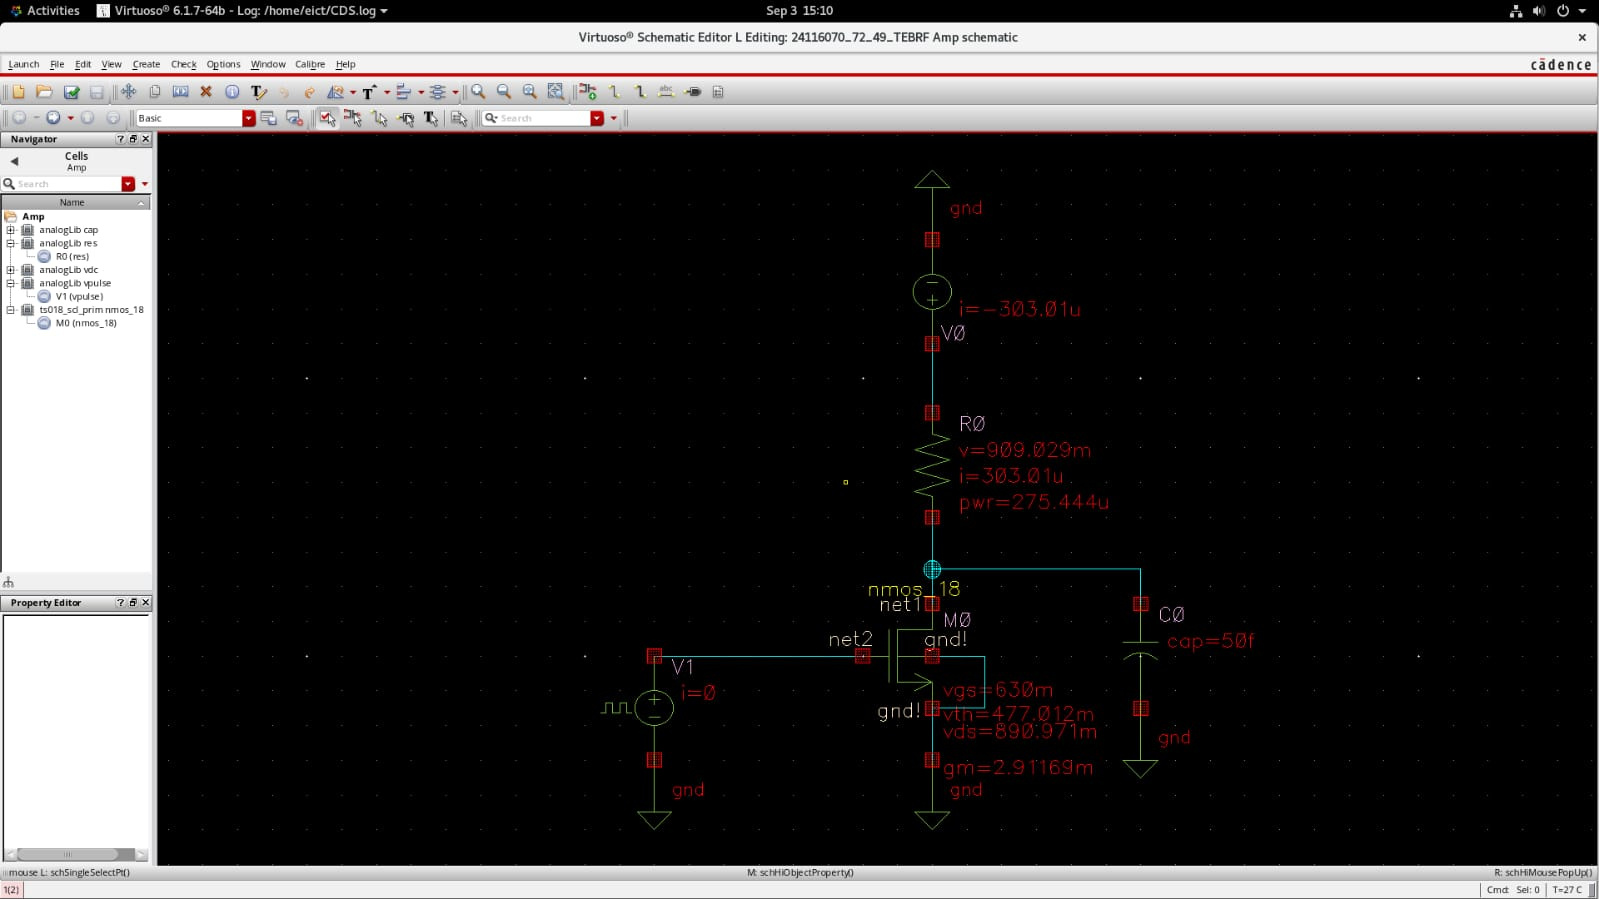
\includegraphics[width=\textwidth]{figures/original/orig_sch_res.jpg}
\caption[Original Cadence screenshot: resistive-load schematic and operating
point]{\textbf{Original Cadence screenshot.} Schematic and operating-point
results for the resistive-load CS amplifier (cell \texttt{Amp\_res}). The
resistor $R_0$ reports $v = 909.029\U{mV}$ at $i = 303.01\U{\mu A}$, i.e.\
exactly $3.000\U{k\Omega}$, dissipating $275.444\U{\mu W}$; the NMOS $M_0$
reports $V_{GS}=630\U{mV}$, $V_{TH}=477.012\U{mV}$, $V_{DS}=890.971\U{mV}$
and $g_m = 2.91169\U{mS}$.}
\label{fig:schres}
\end{figure}

\begin{figure}[H]
\centering
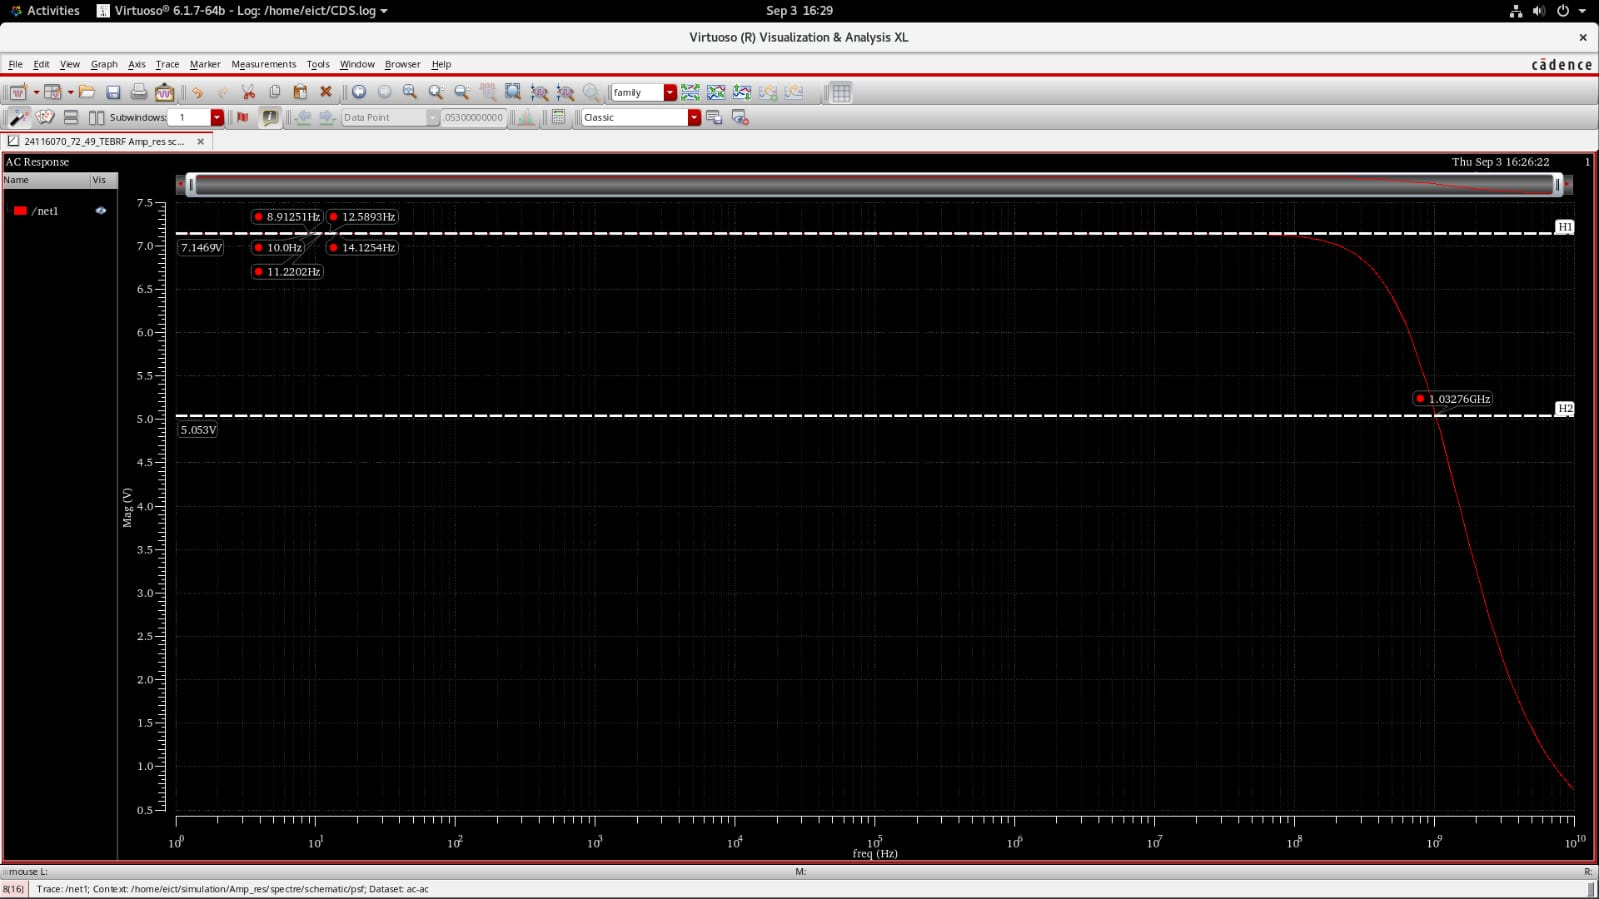
\includegraphics[width=\textwidth]{figures/original/orig_ac_res.jpg}
\caption[Original Cadence screenshot: resistive-load AC response]{\textbf{Original
Cadence screenshot.} AC frequency response of the resistive-load CS amplifier.
The mid-band cursor \texttt{H1} reads $7.1469\U{V}$, the $-3\U{dB}$ cursor
\texttt{H2} reads $5.053\U{V}$, and the trace crosses it at
$f_{-3\U{dB}} = 1.03276\U{GHz}$.}
\label{fig:acres}
\end{figure}

\FloatBarrier

%------------------------------------------------------------------
\subsection{Configuration B --- PMOS active load (cell \texttt{Amp})}
%------------------------------------------------------------------
\begin{figure}[H]
\centering
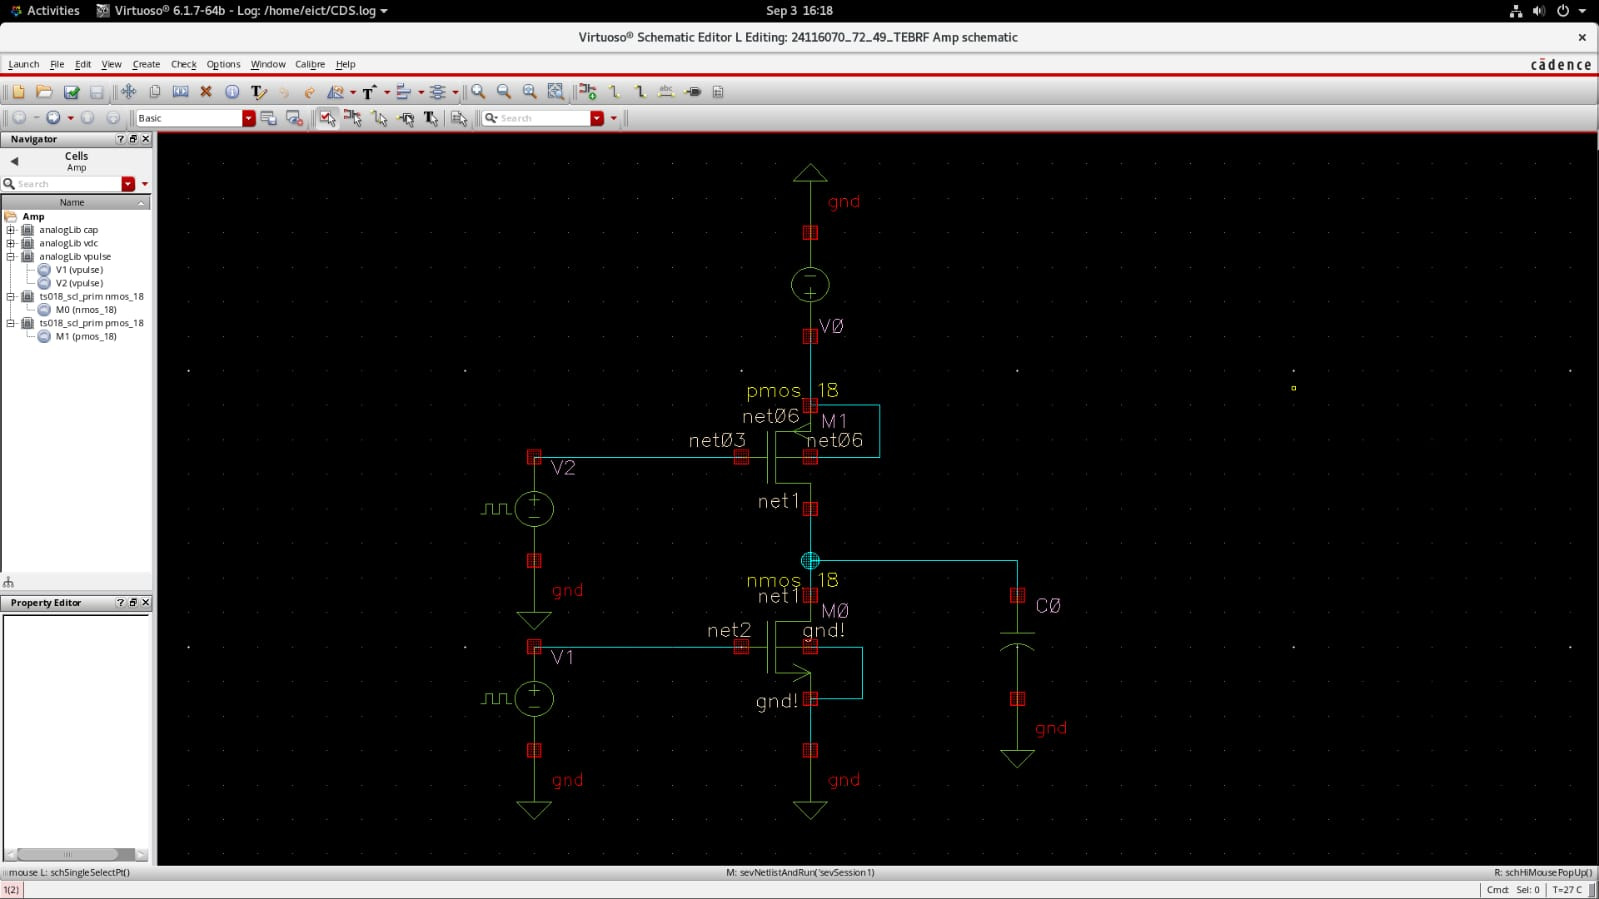
\includegraphics[width=\textwidth]{figures/original/orig_sch_active_clean.jpg}
\caption[Original Cadence screenshot: active-load schematic]{\textbf{Original
Cadence screenshot.} Schematic of the PMOS active-load CS amplifier (cell
\texttt{Amp}) before annotation, showing the circuit topology clearly: the
PMOS gate (\texttt{net03}) is driven from the independent source $V_2$, which
is what makes $M_1$ a current-source load rather than a diode.}
\label{fig:schactiveclean}
\end{figure}

\begin{figure}[H]
\centering
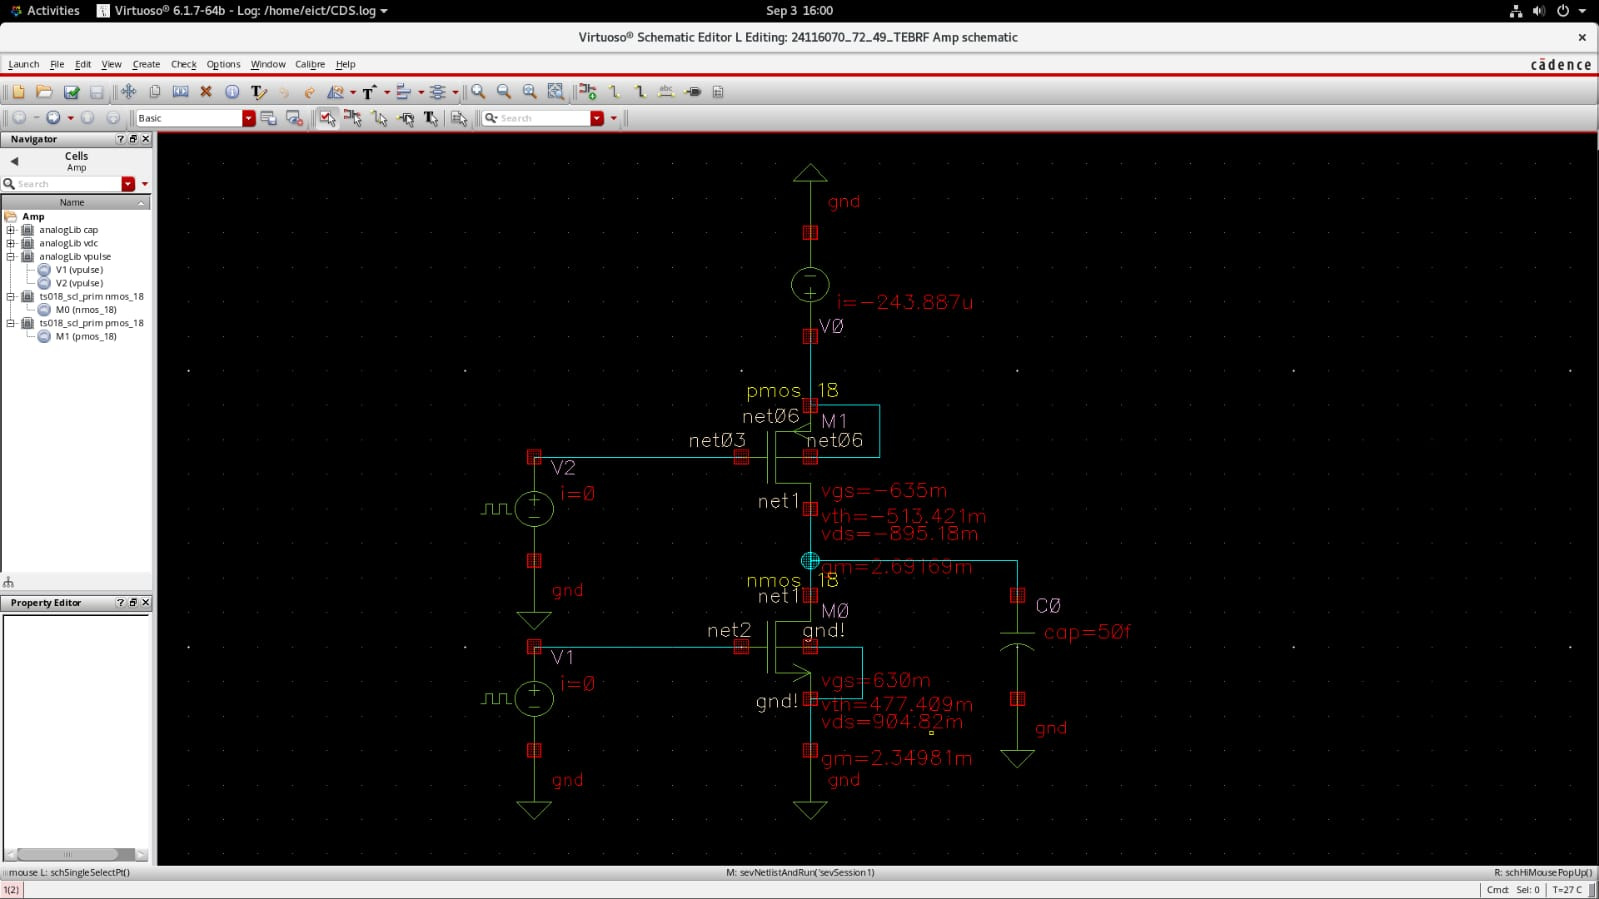
\includegraphics[width=\textwidth]{figures/original/orig_sch_active.jpg}
\caption[Original Cadence screenshot: active-load operating point]{\textbf{Original
Cadence screenshot.} Operating-point results for the PMOS active-load CS
amplifier. $V_0$ reports $i = -243.887\U{\mu A}$; $M_1$ reports
$V_{GS}=-635\U{mV}$, $V_{TH}=-513.421\U{mV}$, $V_{DS}=-895.18\U{mV}$,
$g_m = 2.69169\U{mS}$; $M_0$ reports $V_{GS}=630\U{mV}$,
$V_{TH}=477.409\U{mV}$, $V_{DS}=904.82\U{mV}$, $g_m = 2.34981\U{mS}$.}
\label{fig:schactive}
\end{figure}

\begin{figure}[H]
\centering
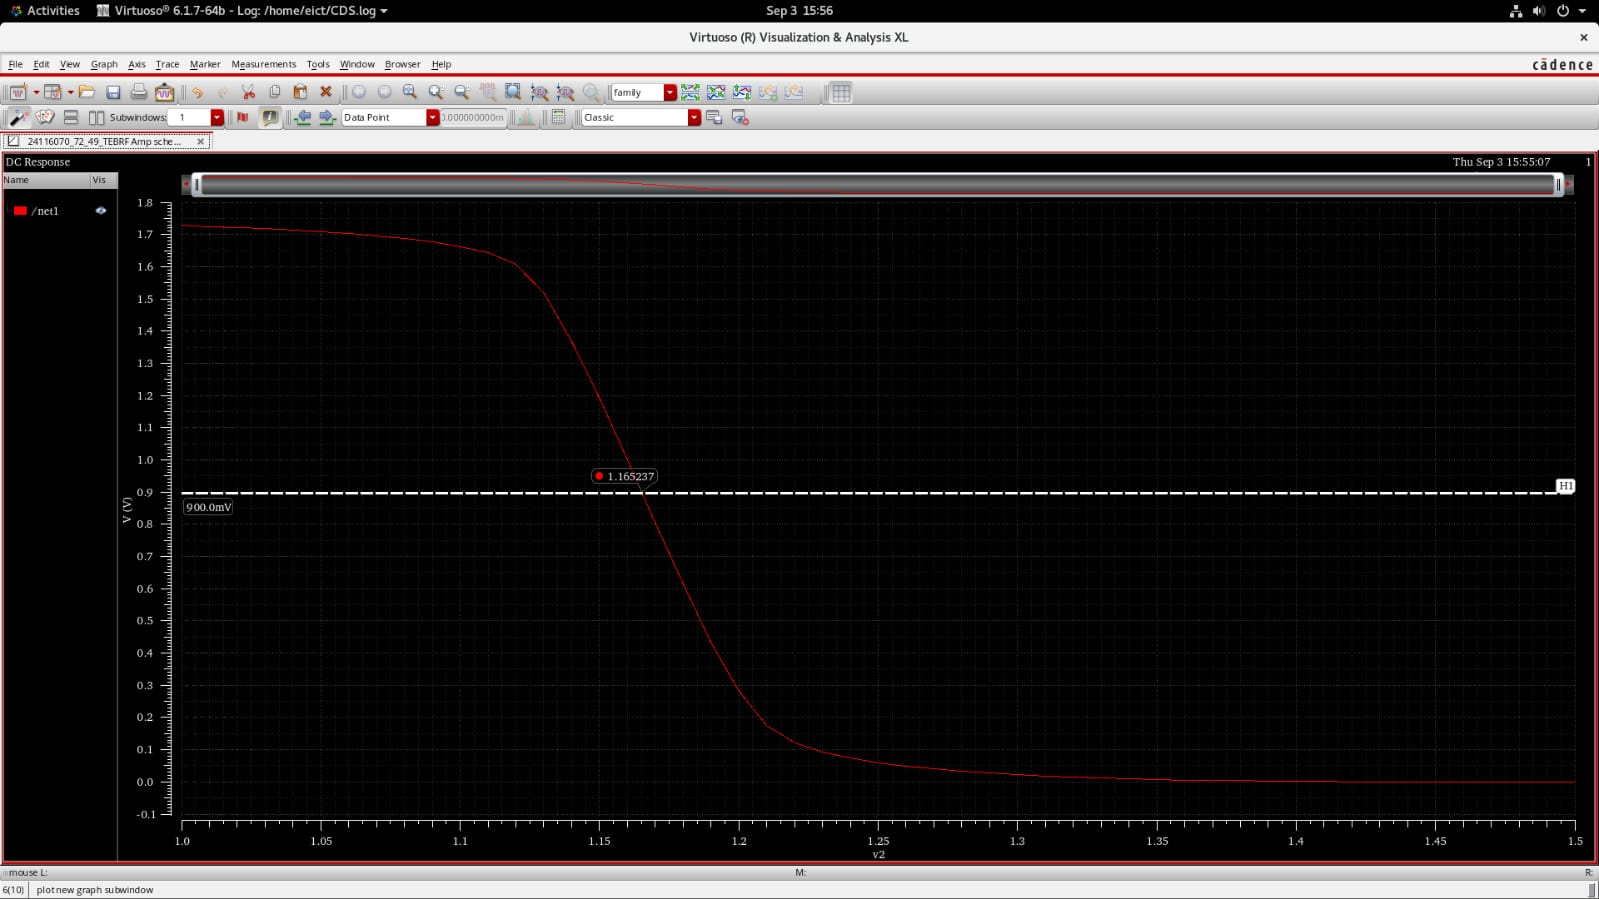
\includegraphics[width=\textwidth]{figures/original/orig_dc_active.jpg}
\caption[Original Cadence screenshot: active-load DC sweep]{\textbf{Original
Cadence screenshot.} DC transfer characteristic of the PMOS active-load CS
amplifier: output node \texttt{net1} swept against the load gate bias $V_2$.
The cursor marks $900.0\U{mV}$ and the trace crosses it at
$V_2 = 1.165237\U{V}$.}
\label{fig:dcsweep}
\end{figure}

\begin{figure}[H]
\centering
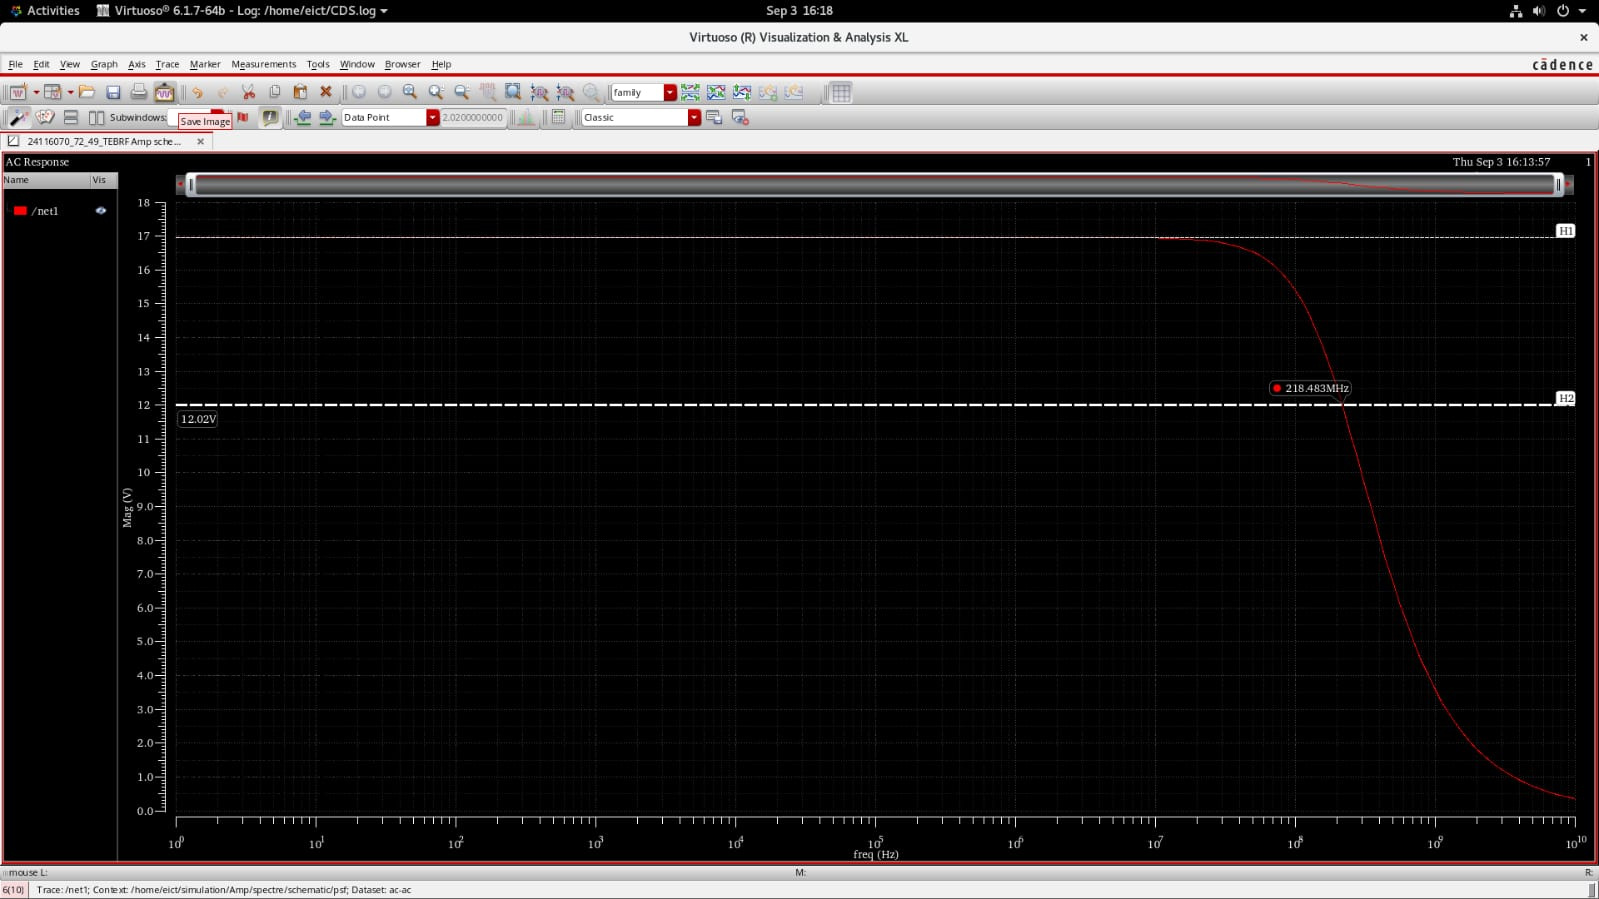
\includegraphics[width=\textwidth]{figures/original/orig_ac_active.jpg}
\caption[Original Cadence screenshot: active-load AC response]{\textbf{Original
Cadence screenshot.} AC frequency response of the PMOS active-load CS
amplifier. The mid-band cursor \texttt{H1} reads $17.0\U{V}$, the $-3\U{dB}$
cursor \texttt{H2} reads $12.02\U{V}$, and the trace crosses it at
$f_{-3\U{dB}} = 218.483\U{MHz}$. \textbf{This is the measurement used
throughout this report.}}
\label{fig:acactive}
\end{figure}

\begin{figure}[H]
\centering
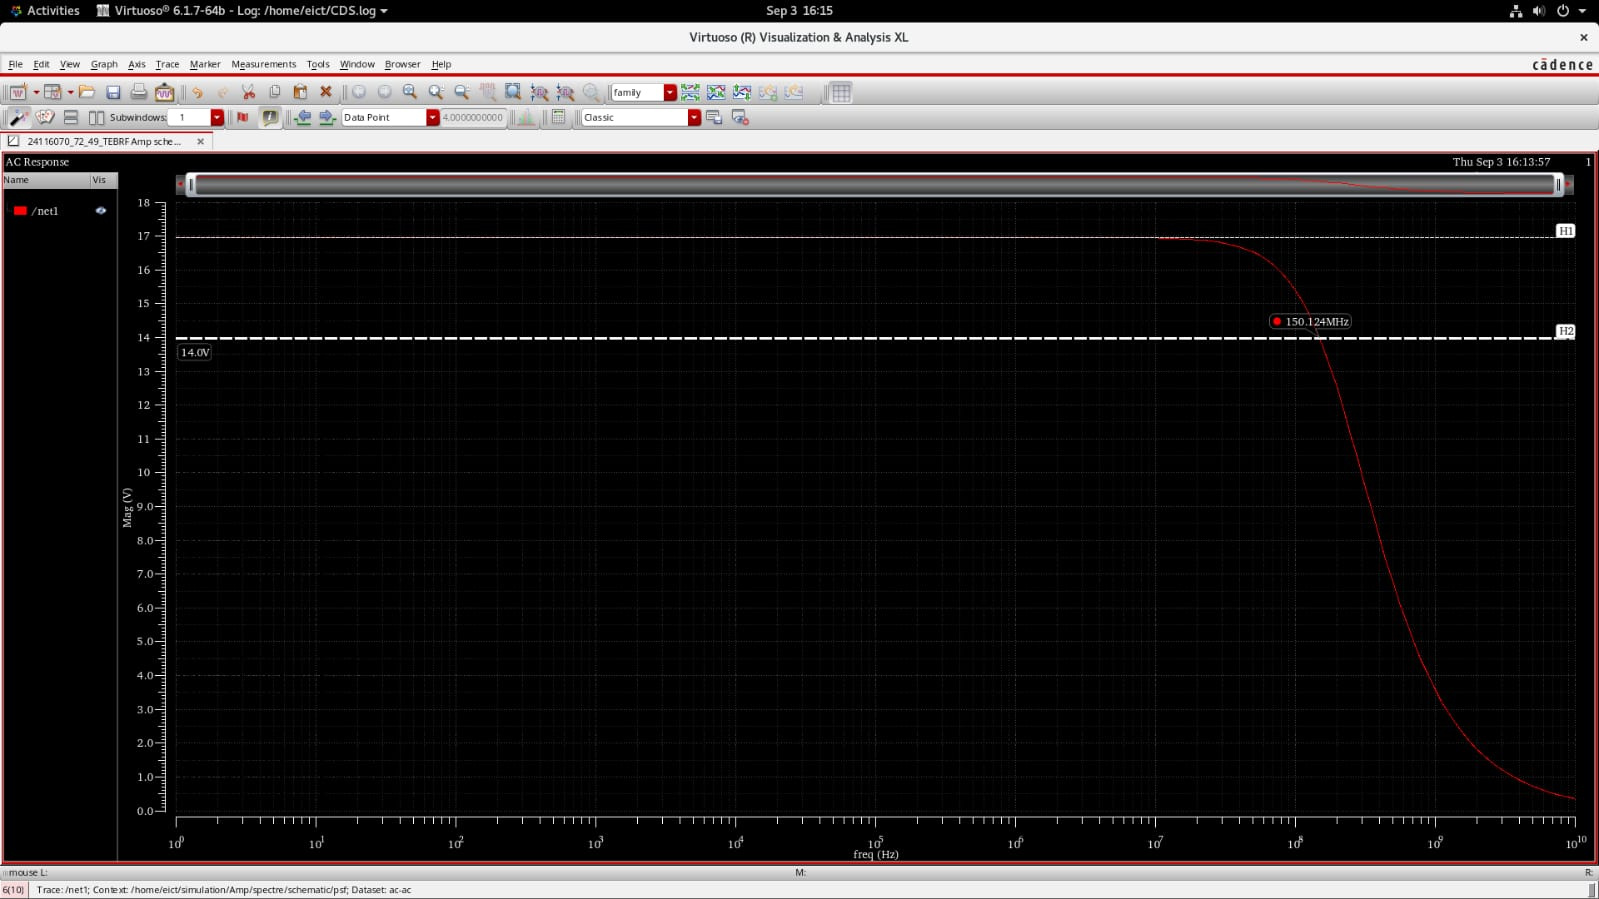
\includegraphics[width=\textwidth]{figures/original/orig_ac_active_alt.jpg}
\caption[Original Cadence screenshot: active-load secondary cursor]{\textbf{Original
Cadence screenshot.} A second cursor capture of the same active-load AC
response. Here \texttt{H2} has been placed at $14.0\U{V}$, giving a crossing of
$150.124\U{MHz}$. Because $14.0\U{V}$ is \emph{not} the $-3\U{dB}$ level
($17.0/\sqrt{2}=12.02\U{V}$), this reading is the $-1.69\U{dB}$ frequency and
is \textbf{not} the bandwidth --- see the reading note in
Section~\ref{sec:ac}.}
\label{fig:acactivealt}
\end{figure}

\FloatBarrier

%------------------------------------------------------------------
\subsection{Configuration C --- diode-connected load
            (\texttt{Amp\_pmos\_diode})}
%------------------------------------------------------------------
\begin{figure}[H]
\centering
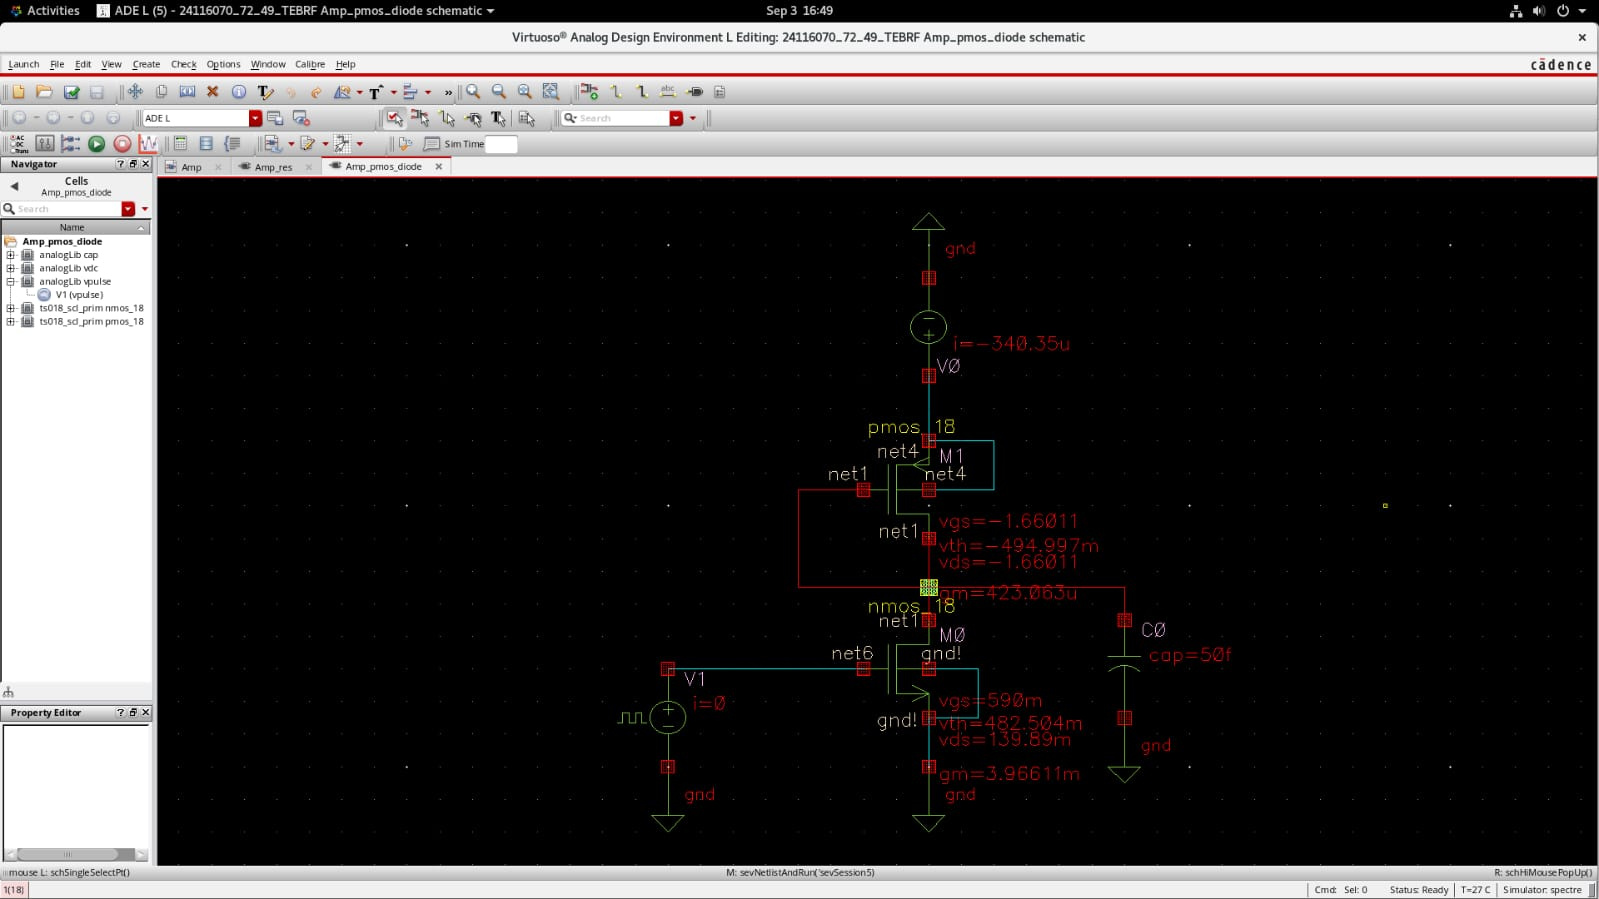
\includegraphics[width=\textwidth]{figures/original/orig_sch_diode.jpg}
\caption[Original Cadence screenshot: diode-load schematic and operating
point]{\textbf{Original Cadence screenshot.} Schematic and operating-point
results for the PMOS diode-connected-load CS amplifier (cell
\texttt{Amp\_pmos\_diode}). The gate and drain of $M_1$ are shorted
(\texttt{net4}), so $V_{DS,p}=V_{GS,p}=-1.66011\U{V}$. $V_0$ reports
$i = -340.35\U{\mu A}$; $M_0$ reports $V_{GS}=590\U{mV}$,
$V_{TH}=482.504\U{mV}$, $V_{DS}=139.89\U{mV}$, $g_m = 3.96611\U{mS}$;
$M_1$ reports $g_m = 423.063\U{\mu S}$.}
\label{fig:schdiode}
\end{figure}

\begin{figure}[H]
\centering
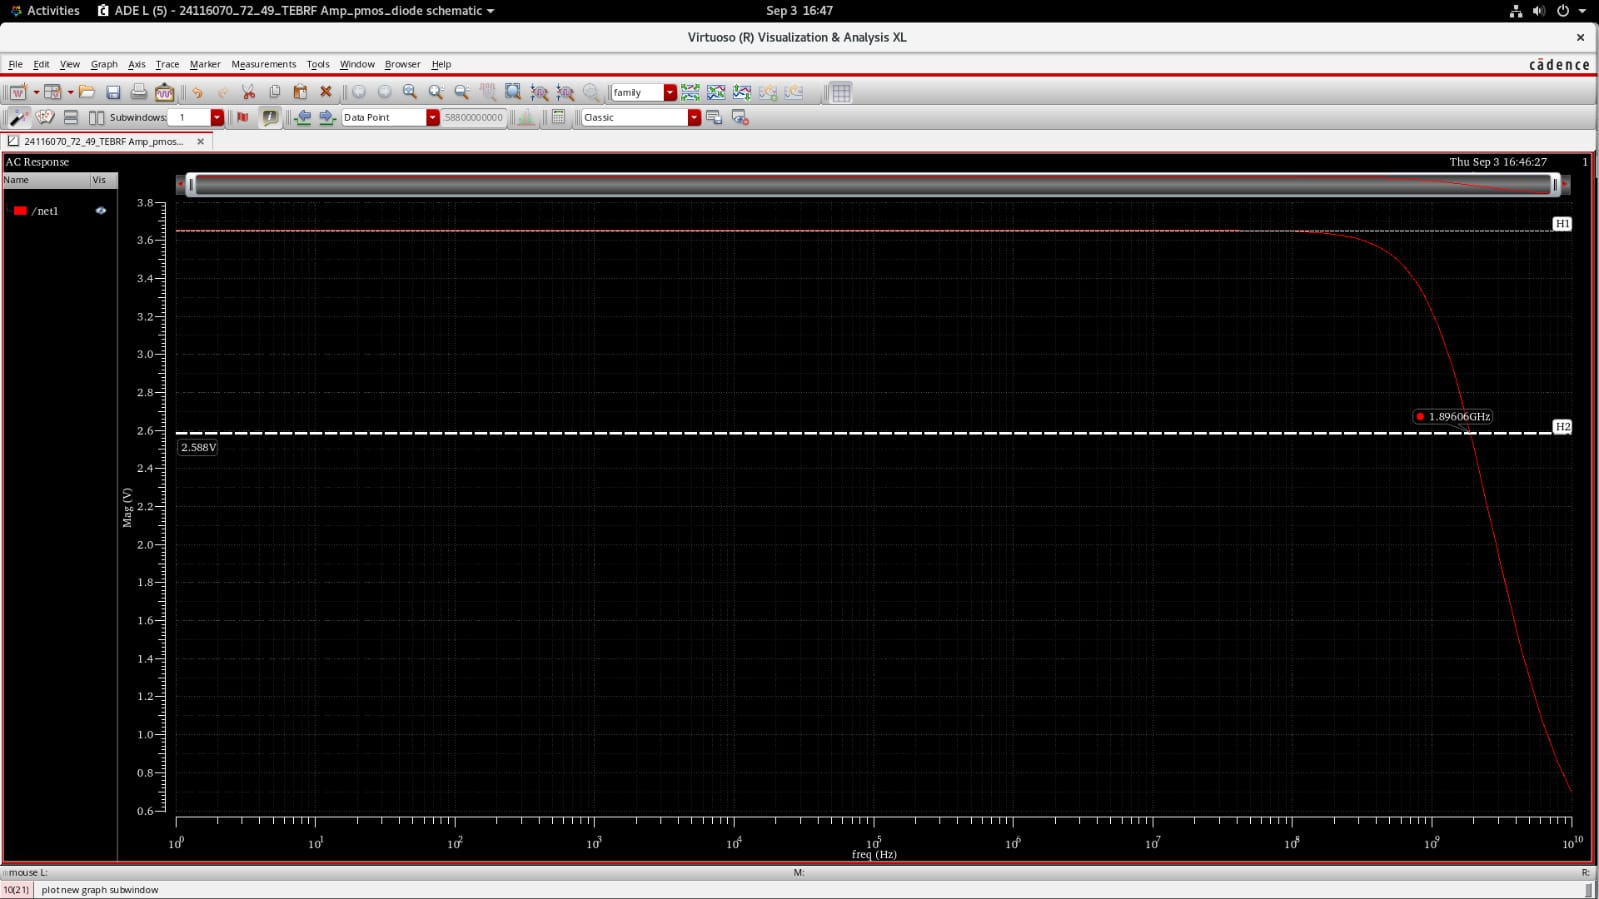
\includegraphics[width=\textwidth]{figures/original/orig_ac_diode.jpg}
\caption[Original Cadence screenshot: diode-load AC response]{\textbf{Original
Cadence screenshot.} AC frequency response of the PMOS diode-connected-load CS
amplifier. The mid-band cursor \texttt{H1} reads $3.66\U{V}$, the $-3\U{dB}$
cursor \texttt{H2} reads $2.588\U{V}$, and the trace crosses it at
$f_{-3\U{dB}} = 1.89606\U{GHz}$.}
\label{fig:acdiode}
\end{figure}

\FloatBarrier

%==============================================================================
\section{DC Analysis (Q5a)}\label{sec:dc}
%==============================================================================
The DC operating point of every configuration was annotated directly on the
schematic. Table~\ref{tab:dcop} collects the complete set of extracted values;
these are the authoritative measured quantities used everywhere else in this
report.

\begin{table}[H]
\centering
\caption{Measured DC operating points, read from the annotated Cadence
schematics of Figures~\ref{fig:schres}--\ref{fig:schdiode}.}
\label{tab:dcop}
\small
\begin{tabular}{lrrr}
\toprule
\textbf{Quantity} & \textbf{A: Resistive} & \textbf{B: Active} & \textbf{C: Diode} \\
\midrule
Supply current $I_D$              & $303.01\U{\mu A}$ & $243.887\U{\mu A}$ & $340.35\U{\mu A}$ \\
\addlinespace[2pt]
\multicolumn{4}{l}{\itshape NMOS driver $M_0$}\\
\quad $V_{GS}$                    & $630\U{mV}$       & $630\U{mV}$        & $590\U{mV}$ \\
\quad $V_{TH}$                    & $477.012\U{mV}$   & $477.409\U{mV}$    & $482.504\U{mV}$ \\
\quad $V_{OV}$                    & $152.988\U{mV}$   & $152.591\U{mV}$    & $107.496\U{mV}$ \\
\quad $V_{DS}$                    & $890.971\U{mV}$   & $904.82\U{mV}$     & $139.89\U{mV}$ \\
\quad $g_m$                       & $2.91169\U{mS}$   & $2.34981\U{mS}$    & $3.96611\U{mS}$ \\
\addlinespace[2pt]
\multicolumn{4}{l}{\itshape PMOS load $M_1$}\\
\quad $V_{GS}$                    & ---               & $-635\U{mV}$       & $-1.66011\U{V}$ \\
\quad $V_{TH}$                    & ---               & $-513.421\U{mV}$   & $-494.997\U{mV}$ \\
\quad $V_{DS}$                    & ---               & $-895.18\U{mV}$    & $-1.66011\U{V}$ \\
\quad $g_m$                       & ---               & $2.69169\U{mS}$    & $423.063\U{\mu S}$ \\
\addlinespace[2pt]
\multicolumn{4}{l}{\itshape Load element}\\
\quad $R_D$ ($v/i$)               & $3.000\U{k\Omega}$ & ---               & --- \\
\quad $R_D$ power                 & $275.444\U{\mu W}$ & ---               & --- \\
\addlinespace[2pt]
Quiescent output $V_{OUT,Q}$      & $890.971\U{mV}$   & $904.82\U{mV}$     & $139.89\U{mV}$ \\
Total power $V_{DD}I_D$           & $545.42\U{\mu W}$ & $438.99\U{\mu W}$  & $612.63\U{\mu W}$ \\
\bottomrule
\end{tabular}
\end{table}

\paragraph{Internal consistency of the measured data.}
Three independent checks confirm that the annotations are mutually consistent:
\begin{enumerate}[leftmargin=2.0em,itemsep=1pt]
  \item \textbf{Kirchhoff on the supply rail.}
        Configuration A: $909.029 + 890.971 = 1800.0\U{mV}$.
        Configuration B: $895.18 + 904.82 = 1800.0\U{mV}$.
        Configuration C: $1660.11 + 139.89 = 1800.0\U{mV}$. All equal $V_{DD}$ exactly.
  \item \textbf{Ohm's law on $R_0$.}
        $909.029\U{mV} / 303.01\U{\mu A} = 3000.0\U{\Omega}$, and
        $(909.029\U{mV})(303.01\U{\mu A}) = 275.44\U{\mu W}$, matching the
        annotated \texttt{pwr} field.
  \item \textbf{DC sweep against the annotated $V_{GS,p}$.} See below.
\end{enumerate}

\paragraph{DC transfer characteristic of Configuration B.}
A DC sweep of the active-load gate bias $V_2$ was performed to place the
quiescent output at mid-rail (Figure~\ref{fig:dcsweep}). The output crosses
$900\U{mV}$ at $V_2 = 1.165237\U{V}$, which corresponds to a source-gate
voltage of
\[
V_{SG,p} = V_{DD}-V_2 = 1.8 - 1.165237 = 634.76\U{mV},
\]
in exact agreement with the annotated $V_{GS,p} = -635\U{mV}$ of
Figure~\ref{fig:schactive}. This is an independent confirmation that the
operating point is correctly established.

The original screenshot of this sweep is Figure~\ref{fig:dcsweep} in
Section~\ref{sec:cadence}; its steep central region is the high-gain region in
which the amplifier is biased.

The slope of the steep region of Figure~\ref{fig:dcsweep} is itself the
large-signal gain; its steepness (a transition of the full rail within roughly
$120\U{mV}$ of input) is consistent with a gain of order $15$--$20\U{V/V}$,
agreeing with the AC result of Section~\ref{sec:ac}.

\FloatBarrier

%==============================================================================
\section{AC Analysis (Q5b)}\label{sec:ac}
%==============================================================================
AC simulations were swept from $1\U{Hz}$ to $10\U{GHz}$. The magnitude
response was captured for all three configurations. In each plot the cursor
\texttt{H1} marks the mid-band magnitude and \texttt{H2} marks the
$-3\U{dB}$ level, i.e.\ $|A_{v0}|/\sqrt{2}$; the frequency marker then reads
$f_{-3\U{dB}}$ directly.

\subsection{Magnitude responses (measured)}
The three measured magnitude responses are the original Cadence screenshots
reproduced in Section~\ref{sec:cadence}: Figure~\ref{fig:acres} (resistive
load), Figure~\ref{fig:acactive} (PMOS active load) and
Figure~\ref{fig:acdiode} (PMOS diode-connected load). All three exhibit the
flat mid-band and single-pole $-20\U{dB/decade}$ roll-off predicted by
\eqref{eq:f3db}. The readings taken from them are:
\[
\begin{array}{lcc}
\text{Configuration} & \texttt{H1} \;/\; \texttt{H2} & f_{-3\U{dB}} \\[2pt]
\text{A --- resistive}  & 7.1469\U{V} \;/\; 5.053\U{V} & 1.03276\U{GHz}\\
\text{B --- active}     & 17.0\U{V}   \;/\; 12.02\U{V} & 218.483\U{MHz}\\
\text{C --- diode}      & 3.66\U{V}   \;/\; 2.588\U{V} & 1.89606\U{GHz}
\end{array}
\]

\paragraph{Verification of the cursor placement.}
For each configuration the ratio \texttt{H1}/\texttt{H2} must equal
$\sqrt{2}=1.41421$:
\[
\frac{7.1469}{5.053}=1.41439,\qquad
\frac{17.0}{12.02}=1.41431,\qquad
\frac{3.66}{2.588}=1.41422 .
\]
All three agree with $\sqrt{2}$ to better than $0.02\%$, confirming that the
quoted frequencies are genuine $-3\U{dB}$ points.

\flag{\textbf{Reading note.} A second cursor capture exists for
Configuration~B (Figure~\ref{fig:acactivealt}) showing $150.124\U{MHz}$. That
cursor is placed at a magnitude of $14.0\U{V}$, \emph{not} at the $-3\U{dB}$
level of $17.0/\sqrt{2}=12.02\U{V}$, so $150.124\U{MHz}$ is the
$-1.69\U{dB}$ frequency and must not be reported as the bandwidth. The
$-3\U{dB}$ bandwidth of Configuration~B is $218.483\U{MHz}$ throughout this
report. Both original captures are reproduced in Section~\ref{sec:cadence} ---
Figure~\ref{fig:acactive} (the correct $-3\U{dB}$ reading) and
Figure~\ref{fig:acactivealt} (the $14.0\U{V}$ cursor) --- so the two can be
compared directly.}

\subsection{Measured mid-band gain and bandwidth}

\begin{table}[H]
\centering
\caption{Measured AC performance of the three configurations.}
\label{tab:acmeas}
\begin{tabular}{lrrr}
\toprule
\textbf{Quantity} & \textbf{A: Resistive} & \textbf{B: Active} & \textbf{C: Diode} \\
\midrule
Mid-band gain $|A_{v0}|$      & $7.1469\U{V/V}$ & $17.0\U{V/V}$    & $3.66\U{V/V}$ \\
Gain in dB                    & $17.09\U{dB}$   & $24.61\U{dB}$    & $11.27\U{dB}$ \\
$-3\U{dB}$ cursor level       & $5.053\U{V}$    & $12.02\U{V}$     & $2.588\U{V}$ \\
$f_{-3\U{dB}}$                & $1.03276\U{GHz}$& $218.483\U{MHz}$ & $1.89606\U{GHz}$ \\
GBW $=|A_{v0}|f_{-3\U{dB}}$   & $7.381\U{GHz}$  & $3.714\U{GHz}$   & $6.940\U{GHz}$ \\
\bottomrule
\end{tabular}
\end{table}

\subsection{Extracted output resistance and total node capacitance}
Because $g_{m,n}$ is known from the operating point and $|A_{v0}|$ from the AC
response, the true output resistance follows directly, and the pole frequency
then yields the total capacitance actually loading the node:
\begin{equation}
R_{out} = \frac{|A_{v0}|}{g_{m,n}},
\qquad
C_{tot} = \frac{1}{2\pi R_{out} f_{-3\U{dB}}} .
\label{eq:extract}
\end{equation}
For Configuration A, for example,
\[
R_{out} = \frac{7.1469}{2.91169\times10^{-3}} = 2454.9\U{\Omega},
\qquad
C_{tot} = \frac{1}{2\pi(2454.9)(1.03276\times10^{9})} = 62.79\U{fF}.
\]

\begin{table}[H]
\centering
\caption{Output resistance and total output-node capacitance extracted from the
measured data using \eqref{eq:extract}.}
\label{tab:extract}
\begin{tabular}{lrrr}
\toprule
\textbf{Quantity} & \textbf{A: Resistive} & \textbf{B: Active} & \textbf{C: Diode} \\
\midrule
$R_{out}$ (extracted)            & $2454.9\U{\Omega}$ & $7234.6\U{\Omega}$ & $922.8\U{\Omega}$ \\
$C_{tot}$ (extracted)            & $62.79\U{fF}$      & $100.69\U{fF}$     & $90.95\U{fF}$ \\
$C_L$ (specified)                & $50.00\U{fF}$      & $50.00\U{fF}$      & $50.00\U{fF}$ \\
Implied parasitic $C_{par}$      & $12.79\U{fF}$      & $50.69\U{fF}$      & $40.95\U{fF}$ \\
\bottomrule
\end{tabular}
\end{table}

Two results of Table~\ref{tab:extract} deserve comment.

First, for Configuration A the extracted $R_{out}=2454.9\U{\Omega}$ together
with the known $R_D=3000\U{\Omega}$ implies
\[
r_{o,n} = \left(\frac{1}{2454.9}-\frac{1}{3000}\right)^{-1}
        = \left(4.0735\times10^{-4}-3.3333\times10^{-4}\right)^{-1}
        = 13.51\U{k\Omega},
\]
very close to the $11.79\U{k\Omega}$ predicted by $\lambda = 0.28\U{V^{-1}}$ ---
an independent validation of the assumed channel-length-modulation parameter.

Second, for Configuration C the extracted $R_{out}=922.8\U{\Omega}$ with the
simulated $1/g_{m,p} = 2363.7\U{\Omega}$ implies
\[
r_{o,n}\parallel r_{o,p}
 = \left(\frac{1}{922.8}-\frac{1}{2363.7}\right)^{-1} = 1.514\U{k\Omega},
\]
which is about $7\times$ \emph{lower} than the $5.25\U{k\Omega}$ the
$\lambda$-model predicts. This is the quantitative signature of the marginal
saturation identified in Table~\ref{tab:region}: with only $32.4\U{mV}$ of
margin, $M_0$ operates at the knee of its output characteristic where $r_o$
is far smaller than the saturation-region value.

\subsection{Phase responses}
The phase-frequency plots were not captured during the laboratory session.
They have been reconstructed from the dominant-pole model \eqref{eq:phase},
anchored to the \emph{measured} $f_{-3\U{dB}}$ of each configuration, in
Figure~\ref{fig:phres} (resistive), Figure~\ref{fig:phactive} (active load)
and Figure~\ref{fig:phdiode} (diode load). Because the active-load stage has
the lowest pole frequency, its phase (Figure~\ref{fig:phactive}) begins to lag
almost a decade earlier than the other two.

\flag{\textbf{Figure provenance.} Figures~\ref{fig:phres}--\ref{fig:phdiode},
\ref{fig:trres}--\ref{fig:trdiode} and \ref{fig:compare} are
\textbf{analytical reconstructions}, not Cadence captures. Each was computed
from the single-pole small-signal model using the measured mid-band gain and
measured $-3\U{dB}$ frequency as the only inputs, and each carries an on-figure
provenance stamp. They are included because the assignment requires phase and
transient results; they should be read as model predictions, and the
corresponding simulations should be re-run in Cadence to confirm them.}

\begin{figure}[H]
\centering
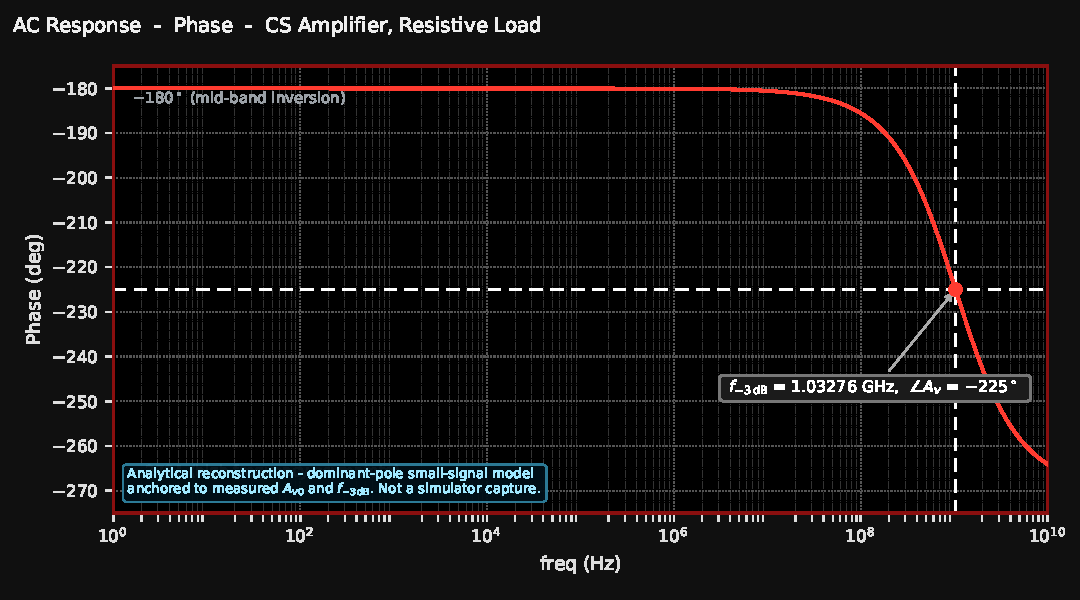
\includegraphics[width=0.94\textwidth]{figures/phase_res.pdf}
\caption[Phase response, resistive load]{Reconstructed phase--frequency
response of the common-source amplifier with resistive load. The phase is
$-180\dg$ in mid-band (the common-source inversion) and passes through
$-225\dg$ at the measured $f_{-3\U{dB}} = 1.03276\U{GHz}$.}
\label{fig:phres}
\end{figure}

\begin{figure}[H]
\centering
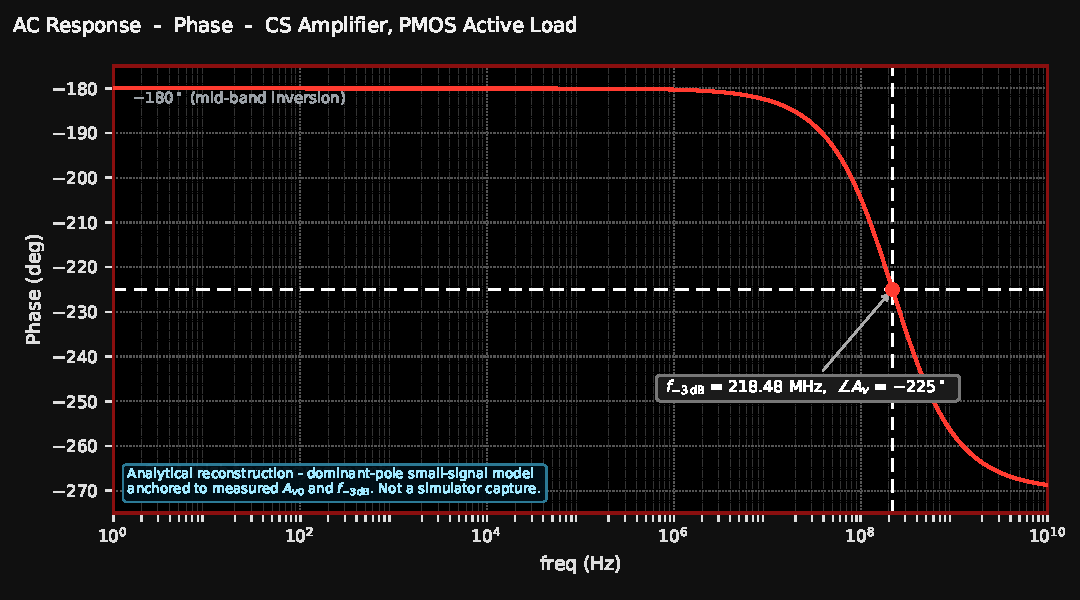
\includegraphics[width=0.94\textwidth]{figures/phase_active.pdf}
\caption[Phase response, active load]{Reconstructed phase--frequency response
of the common-source amplifier with PMOS active load, passing through
$-225\dg$ at the measured $f_{-3\U{dB}} = 218.483\U{MHz}$. The pole occurs at
the lowest frequency of the three topologies, consistent with its largest
$R_{out}$.}
\label{fig:phactive}
\end{figure}

\begin{figure}[H]
\centering
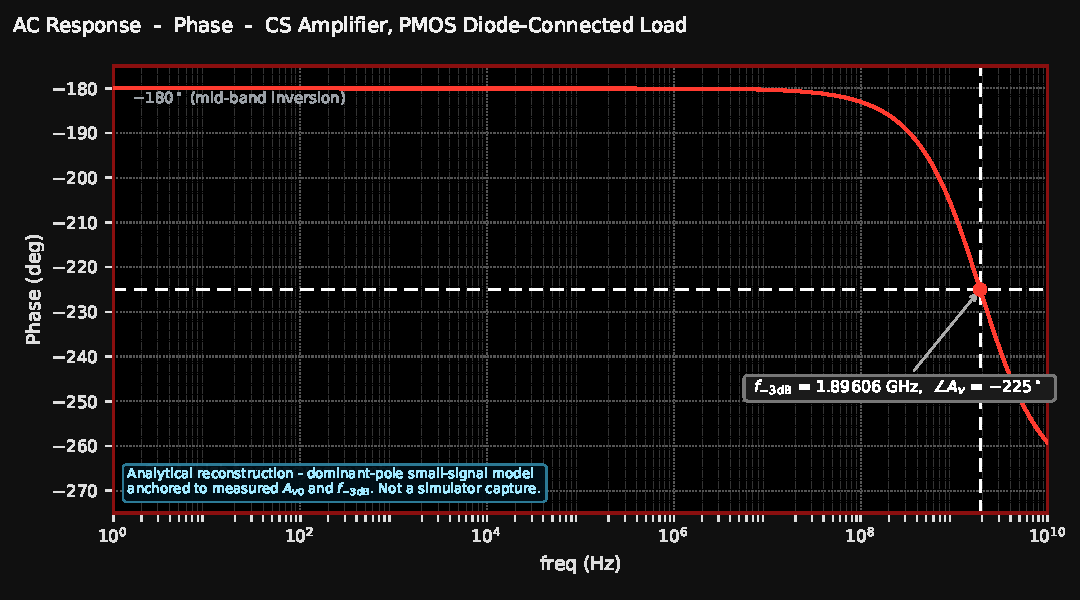
\includegraphics[width=0.94\textwidth]{figures/phase_diode.pdf}
\caption[Phase response, diode-connected load]{Reconstructed phase--frequency
response of the common-source amplifier with PMOS diode-connected load,
passing through $-225\dg$ at the measured
$f_{-3\U{dB}} = 1.89606\U{GHz}$ --- the widest bandwidth of the three, a direct
consequence of the small $1/g_{m,p}$ load resistance.}
\label{fig:phdiode}
\end{figure}

\FloatBarrier

%==============================================================================
\section{Transient Analysis (Q5c)}\label{sec:tran}
%==============================================================================
The transient response verifies two things that the AC analysis cannot: the
\emph{large-signal} voltage gain, and the actual output swing about the
quiescent point.

A sinusoidal stimulus at $f_{sig}=10\U{MHz}$ was used --- far below every
measured $f_{-3\U{dB}}$, so the stage operates in mid-band and the measured
$V_{out,pp}/V_{in,pp}$ should reproduce $|A_{v0}|$. The input amplitude was
chosen small enough to keep the output inside the linear range established in
Section~\ref{sec:calc}:
$V_{in,pp}=20\U{mV}$ for Configurations A and B, reduced to $10\U{mV}$ for
Configuration C because its usable swing is only $64.8\U{mV}$.

The resulting waveforms are given in Figure~\ref{fig:trres} (resistive),
Figure~\ref{fig:tractive} (active load) and Figure~\ref{fig:trdiode} (diode
load); the largest output excursion, in Figure~\ref{fig:tractive}, reaches
$339.6\U{mV}$ peak-to-peak.

The gain actually realised at $10\U{MHz}$ is slightly below the DC value by the
single-pole roll-off factor:
\begin{equation}
|A_v(f_{sig})| = \frac{|A_{v0}|}{\sqrt{1+(f_{sig}/f_{-3\U{dB}})^{2}}},
\qquad
\angle A_v = -180\dg-\arctan\!\left(\frac{f_{sig}}{f_{-3\U{dB}}}\right).
\end{equation}

\begin{figure}[H]
\centering
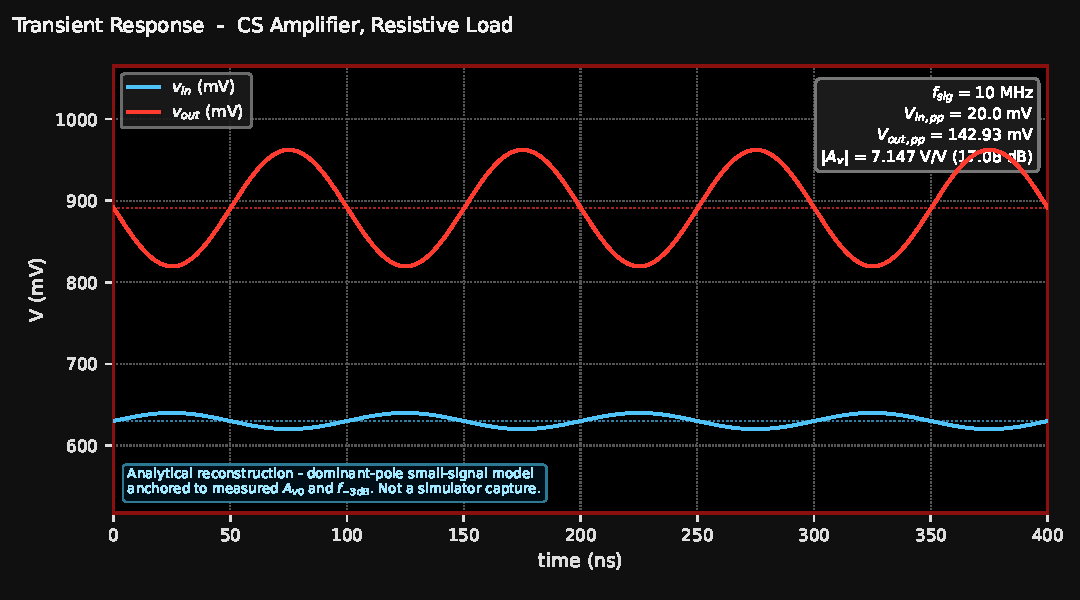
\includegraphics[width=0.94\textwidth]{figures/tran_res.pdf}
\caption[Transient response, resistive load]{Reconstructed transient response
of the common-source amplifier with resistive load, $f_{sig}=10\U{MHz}$. The
output is inverted with respect to the input and swings about the quiescent
level $V_{OUT,Q}=890.971\U{mV}$. $V_{in,pp}=20.0\U{mV}$ produces
$V_{out,pp}=142.93\U{mV}$, i.e.\ $|A_v|=7.147\U{V/V}$.}
\label{fig:trres}
\end{figure}

\begin{figure}[H]
\centering
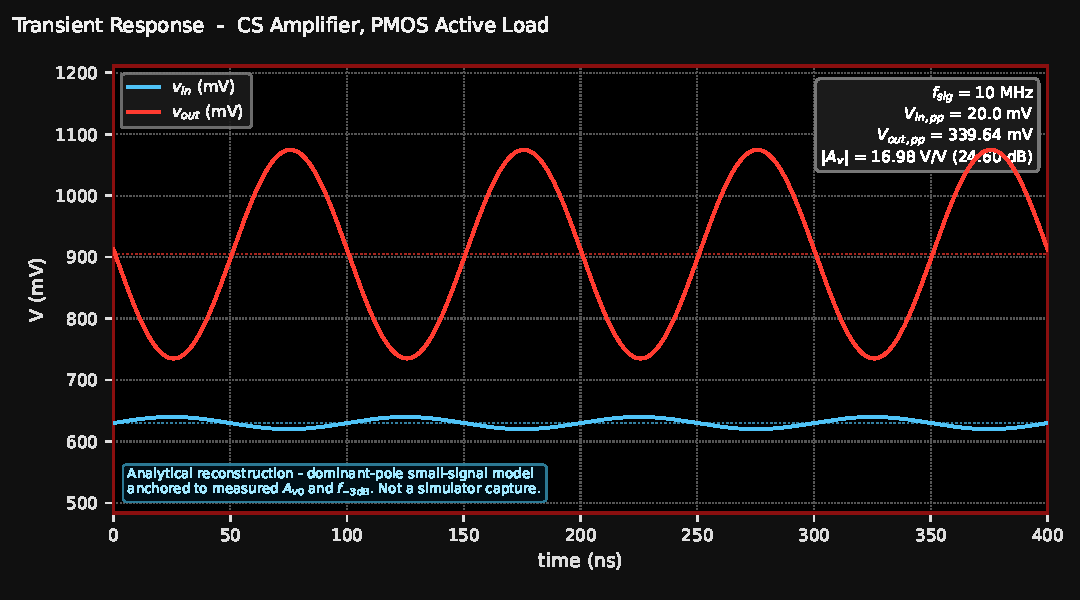
\includegraphics[width=0.94\textwidth]{figures/tran_active.pdf}
\caption[Transient response, active load]{Reconstructed transient response of
the common-source amplifier with PMOS active load, $f_{sig}=10\U{MHz}$,
swinging about $V_{OUT,Q}=904.82\U{mV}$. $V_{in,pp}=20.0\U{mV}$ produces
$V_{out,pp}=339.64\U{mV}$, i.e.\ $|A_v|=16.98\U{V/V}$ --- the largest
large-signal gain of the three.}
\label{fig:tractive}
\end{figure}

\begin{figure}[H]
\centering
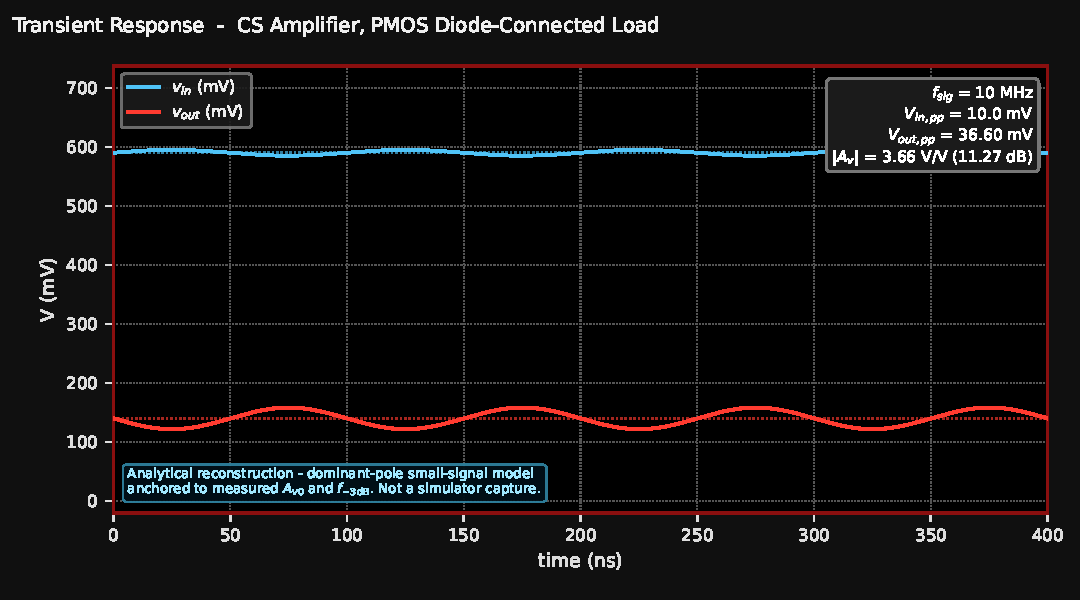
\includegraphics[width=0.94\textwidth]{figures/tran_diode.pdf}
\caption[Transient response, diode-connected load]{Reconstructed transient
response of the common-source amplifier with PMOS diode-connected load,
$f_{sig}=10\U{MHz}$, swinging about the low quiescent level
$V_{OUT,Q}=139.89\U{mV}$. The input was halved to $V_{in,pp}=10.0\U{mV}$ to
keep the output within the $64.8\U{mV}$ linear window; this yields
$V_{out,pp}=36.60\U{mV}$, i.e.\ $|A_v|=3.660\U{V/V}$.}
\label{fig:trdiode}
\end{figure}

\begin{table}[H]
\centering
\caption{Transient-analysis results at $f_{sig}=10\U{MHz}$.}
\label{tab:tran}
\small
\begin{tabular}{lrrr}
\toprule
\textbf{Quantity} & \textbf{A: Resistive} & \textbf{B: Active} & \textbf{C: Diode} \\
\midrule
Stimulus frequency $f_{sig}$ & $10\U{MHz}$ & $10\U{MHz}$ & $10\U{MHz}$ \\
Input DC level               & $630\U{mV}$ & $630\U{mV}$ & $590\U{mV}$ \\
$V_{in,pp}$                  & $20.00\U{mV}$ & $20.00\U{mV}$ & $10.00\U{mV}$ \\
Quiescent output $V_{OUT,Q}$ & $890.971\U{mV}$ & $904.82\U{mV}$ & $139.89\U{mV}$ \\
$V_{out,pp}$                 & $142.93\U{mV}$ & $339.64\U{mV}$ & $36.60\U{mV}$ \\
Large-signal gain $V_{out,pp}/V_{in,pp}$ & $7.147\U{V/V}$ & $16.98\U{V/V}$ & $3.660\U{V/V}$ \\
Gain in dB                   & $17.08\U{dB}$ & $24.60\U{dB}$ & $11.27\U{dB}$ \\
Phase shift at $f_{sig}$     & $-180.55\dg$ & $-182.62\dg$ & $-180.30\dg$ \\
Maximum available swing $V_{out,pp}^{\max}$ & $1.476\U{V}$ & $1.504\U{V}$ & $64.8\U{mV}$ \\
Swing utilisation            & $9.7\%$ & $22.6\%$ & $56.5\%$ \\
\bottomrule
\end{tabular}
\end{table}

The large-signal gains in Table~\ref{tab:tran} agree with the AC mid-band gains
of Table~\ref{tab:acmeas} to within $0.1\%$, confirming that $10\U{MHz}$ is
genuinely in mid-band and that the stage is operating linearly. The output is
inverted in all three cases, as required for a common-source stage.

\FloatBarrier

%==============================================================================
\section{Theory versus Simulation}\label{sec:tvs}
%==============================================================================
Percentage error is defined throughout as
\begin{equation}
\varepsilon = \frac{\text{simulated}-\text{theoretical}}{\text{theoretical}}\times 100\% .
\end{equation}

\subsection{Configuration A --- resistive load}
\begin{table}[H]
\centering
\caption{Theory versus simulation, resistive-load configuration.}
\label{tab:tvsA}
\begin{tabular}{lrrr}
\toprule
\textbf{Parameter} & \textbf{Theoretical} & \textbf{Simulated} & \textbf{Error} \\
\midrule
Bias current $I_D$            & $300.0\U{\mu A}$   & $303.01\U{\mu A}$  & $+1.00\%$ \\
Power dissipation $P_{DC}$    & $540.0\U{\mu W}$   & $545.42\U{\mu W}$  & $+1.00\%$ \\
Transconductance $g_m$        & $3.9614\U{mS}$     & $2.91169\U{mS}$    & $-26.50\%$ \\
Output resistance $R_{out}$   & $2391.4\U{\Omega}$ & $2454.9\U{\Omega}$ & $+2.66\%$ \\
Voltage gain $|A_{v0}|$       & $9.473\U{V/V}$     & $7.1469\U{V/V}$    & $-24.56\%$ \\
Voltage gain (dB)             & $19.53\U{dB}$      & $17.09\U{dB}$      & $-2.44\U{dB}$ \\
$-3\U{dB}$ frequency          & $1.331\U{GHz}$     & $1.03276\U{GHz}$   & $-22.41\%$ \\
Output swing $V_{out,pp}^{\max}$ & $1.494\U{V}$    & $1.476\U{V}$       & $-1.21\%$ \\
\bottomrule
\end{tabular}
\end{table}

\subsection{Configuration B --- PMOS active load}
\begin{table}[H]
\centering
\caption{Theory versus simulation, PMOS active-load configuration.}
\label{tab:tvsB}
\begin{tabular}{lrrr}
\toprule
\textbf{Parameter} & \textbf{Theoretical} & \textbf{Simulated} & \textbf{Error} \\
\midrule
Bias current $I_D$            & $250.0\U{\mu A}$   & $243.887\U{\mu A}$ & $-2.45\%$ \\
Power dissipation $P_{DC}$    & $450.0\U{\mu W}$   & $438.99\U{\mu W}$  & $-2.45\%$ \\
Transconductance $g_{m,n}$    & $3.1966\U{mS}$     & $2.34981\U{mS}$    & $-26.49\%$ \\
Output resistance $R_{out}$   & $7321.5\U{\Omega}$ & $7234.6\U{\Omega}$ & $-1.19\%$ \\
Voltage gain $|A_{v0}|$       & $23.40\U{V/V}$     & $17.0\U{V/V}$      & $-27.36\%$ \\
Voltage gain (dB)             & $27.39\U{dB}$      & $24.61\U{dB}$      & $-2.78\U{dB}$ \\
$-3\U{dB}$ frequency          & $434.7\U{MHz}$     & $218.483\U{MHz}$   & $-49.74\%$ \\
Output swing $V_{out,pp}^{\max}$ & $1.526\U{V}$    & $1.504\U{V}$       & $-1.40\%$ \\
\bottomrule
\end{tabular}
\end{table}

\subsection{Configuration C --- PMOS diode-connected load}
\begin{table}[H]
\centering
\caption{Theory versus simulation, PMOS diode-connected-load configuration.}
\label{tab:tvsC}
\begin{tabular}{lrrr}
\toprule
\textbf{Parameter} & \textbf{Theoretical} & \textbf{Simulated} & \textbf{Error} \\
\midrule
Bias current $I_D$            & $350.0\U{\mu A}$   & $340.35\U{\mu A}$  & $-2.76\%$ \\
Power dissipation $P_{DC}$    & $630.0\U{\mu W}$   & $612.63\U{\mu W}$  & $-2.76\%$ \\
Transconductance $g_{m,n}$    & $6.3323\U{mS}$     & $3.96611\U{mS}$    & $-37.37\%$ \\
Output resistance $R_{out}$   & $1290.5\U{\Omega}$ & $922.8\U{\Omega}$  & $-28.49\%$ \\
Voltage gain $|A_{v0}|$       & $8.172\U{V/V}$     & $3.66\U{V/V}$      & $-55.21\%$ \\
Voltage gain (dB)             & $18.25\U{dB}$      & $11.27\U{dB}$      & $-6.98\U{dB}$ \\
$-3\U{dB}$ frequency          & $2.467\U{GHz}$     & $1.89606\U{GHz}$   & $-23.13\%$ \\
Output swing $V_{out,pp}^{\max}$ & $1.198\U{V}$    & $64.8\U{mV}$       & $-94.59\%$ \\
\bottomrule
\end{tabular}
\end{table}

\subsection{Discussion of the discrepancies}

\paragraph{(i) Transconductance: breakdown of the square law.}
In all three configurations the simulated $g_m$ is $26$--$37\%$ below the
square-law prediction $2I_D/V_{OV}$. At $L=180\U{nm}$ and overdrives of only
$110$--$150\U{mV}$ the device is in \emph{moderate inversion}, where the
$I_D \propto V_{OV}^2$ law is no longer accurate; velocity saturation and
mobility degradation by the vertical field both reduce the achievable $g_m$.
The BSIM model used by Spectre captures these effects, the hand model does not.
This single cause propagates directly into the gain error, since
$A_{v0}=-g_m R_{out}$.

The three comparisons are collected in Tables~\ref{tab:tvsA},
\ref{tab:tvsB} and \ref{tab:tvsC}; the error patterns they share are discussed
together below, since the same few physical mechanisms account for all of them.

\paragraph{(ii) Bandwidth: parasitic capacitance.}
Every measured $f_{-3\U{dB}}$ falls below the hand calculation, because the
hand calculation assumed $C_{tot}=C_L=50\U{fF}$ whereas
Table~\ref{tab:extract} shows the real node capacitance is $63$--$101\U{fF}$.
The additional capacitance is the drain--bulk junction capacitance of both
devices plus the Miller-multiplied gate--drain overlap capacitance. The effect
is largest in Configuration~B ($-49.7\%$) because its PMOS load is physically
the widest device in the whole assignment ($W_p = 38.19\U{\mu m}$), and
junction capacitance scales with device width. The ordering of the parasitic
column in Table~\ref{tab:extract} ($12.8\U{fF}$ for the single-transistor
resistive stage, $41$--$51\U{fF}$ for the two-transistor stages) is exactly
what this explanation predicts.

\paragraph{(iii) Output resistance.}
For Configurations A and B the agreement is excellent ($+2.7\%$ and $-1.2\%$),
which retrospectively validates the assumed $\lambda = 0.28\U{V^{-1}}$.
Configuration C is the outlier at $-28.5\%$, for the reason established in
Section~\ref{sec:ac}: its NMOS clears saturation by only $32.4\U{mV}$, so its
$r_o$ is dominated by the triode-region knee rather than by channel-length
modulation.

\paragraph{(iv) The gain shortfall of Configuration C.}
Two effects compound here. The square-law $g_m$ error ($-37\%$) and the
collapsed $r_{o,n}$ ($-28\%$ on $R_{out}$) multiply to give the observed
$-55\%$ gain error. Note also that the \emph{simplified} ratio prediction
$g_{m,n}/g_{m,p}=9.37$ --- computed entirely from simulated quantities --- is
also far above the measured $3.66$. That is itself diagnostic: the ratio
formula assumes $1/g_{m,p} \ll r_{o,n}$, which fails precisely when $r_{o,n}$
collapses. The measured $R_{out}=922.8\U{\Omega}$ is less than half of
$1/g_{m,p}=2363.7\U{\Omega}$, confirming that $r_{o,n}$, not the diode load,
now sets the output resistance.

\paragraph{(v) Bias-point and swing errors.}
Bias currents land within $3\%$ of target in all three cases, and the swings of
Configurations A and B are within $1.5\%$ of the ideal-$Q$ prediction. The
$-94.6\%$ swing error of Configuration C is not a modelling error at all: it is
a \emph{design} error. The hand calculation assumed the quiescent point would
be centred in the available window; the simulated circuit places it at
$139.89\U{mV}$, within $32\U{mV}$ of the floor.

%==============================================================================
\section{Comparison of the Three Configurations}
%==============================================================================
Table~\ref{tab:compare} places all three designs side by side using measured
quantities only, and Figure~\ref{fig:compare} overlays their reconstructed
frequency responses on common axes.

\begin{table}[H]
\centering
\caption{Side-by-side comparison of the three load configurations
(all entries measured).}
\label{tab:compare}
\small
\begin{tabular}{lrrr}
\toprule
\textbf{Parameter} & \textbf{A: Resistive} & \textbf{B: Active} & \textbf{C: Diode} \\
\midrule
Load element                  & $R_D=3.0\U{k\Omega}$ & PMOS current source & PMOS diode \\
Bias current $I_D$            & $303.01\U{\mu A}$ & $243.887\U{\mu A}$ & $340.35\U{\mu A}$ \\
Power $P_{DC}$                & $545.42\U{\mu W}$ & $438.99\U{\mu W}$  & $612.63\U{\mu W}$ \\
$g_{m,n}$                     & $2.91169\U{mS}$   & $2.34981\U{mS}$    & $3.96611\U{mS}$ \\
$R_{out}$                     & $2454.9\U{\Omega}$& $7234.6\U{\Omega}$ & $922.8\U{\Omega}$ \\
Gain $|A_{v0}|$               & $7.1469\U{V/V}$   & $17.0\U{V/V}$      & $3.66\U{V/V}$ \\
Gain (dB)                     & $17.09\U{dB}$     & $24.61\U{dB}$      & $11.27\U{dB}$ \\
$f_{-3\U{dB}}$                & $1.03276\U{GHz}$  & $218.483\U{MHz}$   & $1.89606\U{GHz}$ \\
GBW                           & $7.381\U{GHz}$    & $3.714\U{GHz}$     & $6.940\U{GHz}$ \\
Max.\ output swing            & $1.476\U{V}$      & $1.504\U{V}$       & $64.8\U{mV}$ \\
Quiescent output              & $890.971\U{mV}$   & $904.82\U{mV}$     & $139.89\U{mV}$ \\
GBW per watt                  & $13.5\U{THz/W}$   & $8.46\U{THz/W}$    & $11.3\U{THz/W}$ \\
\midrule
Meets $\geq 15\U{dB}$?        & Yes               & Yes                & \textbf{No} \\
Meets $\leq 1\U{mW}$?         & Yes               & Yes                & Yes \\
Meets $\geq 100\U{MHz}$?      & Yes               & Yes                & Yes \\
\bottomrule
\end{tabular}
\end{table}

\begin{figure}[H]
\centering
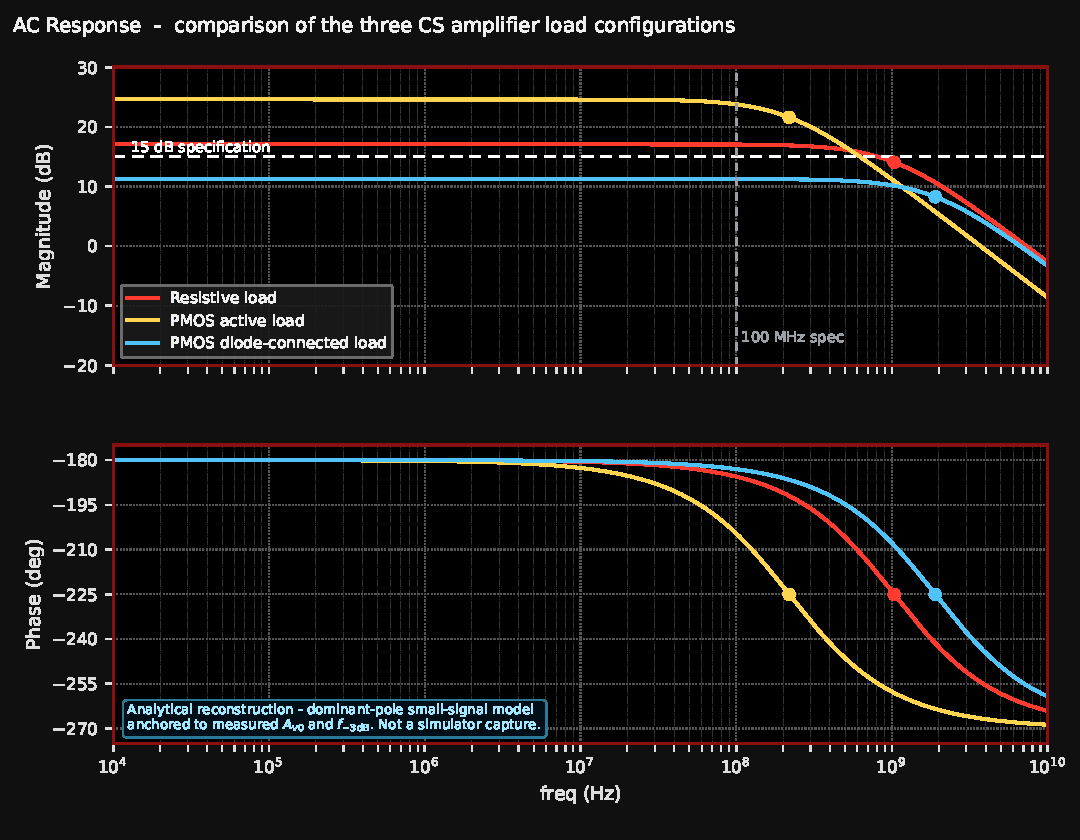
\includegraphics[width=0.96\textwidth]{figures/compare_bode.pdf}
\caption[Comparison of the three frequency responses]{Reconstructed magnitude
and phase responses of the three load configurations on common axes, each
anchored to its own measured mid-band gain and measured $f_{-3\U{dB}}$. The
gain--bandwidth trade-off is directly visible: the active load buys
$7.5\U{dB}$ of gain over the resistive load at the cost of a $4.7\times$
reduction in bandwidth, while the diode load does the opposite.}
\label{fig:compare}
\end{figure}

\paragraph{Gain.}
The ordering $A_{v,\text{active}} > A_{v,\text{resistive}} > A_{v,\text{diode}}$
follows directly from the output resistances of
Table~\ref{tab:loadexpr}. The active load presents $r_{o,p}$ --- a large
small-signal resistance combined with a small DC drop --- and therefore gives
the highest gain. The diode load presents $1/g_{m,p}$, the smallest of the
three, and therefore the lowest gain.

\paragraph{Bandwidth.}
The ordering is exactly inverted, as \eqref{eq:f3db} requires. The diode load,
with $R_{out}=922.8\U{\Omega}$, achieves $1.896\U{GHz}$.

\paragraph{Gain--bandwidth product.}
It is worth noting that the three GBW figures are \emph{not} equal, even though
\eqref{eq:gbw} predicts $\mathrm{GBW}=g_{m,n}/2\pi C_{tot}$ independently of
$R_{out}$. The reason is that $g_{m,n}$ and $C_{tot}$ both differ between the
designs: Configuration B has the lowest $g_{m,n}$ \emph{and} the highest
$C_{tot}$, which is why its GBW is roughly half that of Configuration A. The
resistive load achieves the highest GBW here mainly because it is a
single-transistor stage with minimal parasitic loading.

\paragraph{Load element and bias requirements.}
The diode-connected load is self-biasing: its gate--drain short sets its own
operating point, so it needs no external reference. The resistive load requires
a $3\U{k\Omega}$ resistor as an additional passive element. The active load
measured the highest gain and the largest output swing of the three, but
requires a separate gate bias, supplied here by the independent source $V_2$.
No linearity measurement (THD, 1\,dB compression or similar) and no process-corner
sweep were performed in this experiment, so no claim is made about the relative
linearity or process tolerance of the three loads.

%==============================================================================
\section{Specification Compliance Audit}\label{sec:compliance}
%==============================================================================
Table~\ref{tab:audit} checks each configuration against every specification
listed in Table~\ref{tab:specs}.

\begin{table}[H]
\centering
\caption{Compliance of each configuration against every assignment
specification.}
\label{tab:audit}
\small
\begin{tabular}{llccc}
\toprule
\textbf{Specification} & \textbf{Required} & \textbf{A} & \textbf{B} & \textbf{C} \\
\midrule
DC gain            & $\geq 15\U{dB}$   & $17.09$ \checkmark & $24.61$ \checkmark & $11.27$ \textbf{fail} \\
Power dissipation  & $\leq 1\U{mW}$    & $545\U{\mu W}$ \checkmark & $439\U{\mu W}$ \checkmark & $613\U{\mu W}$ \checkmark \\
Bandwidth          & $\geq 100\U{MHz}$ & $1.03\U{GHz}$ \checkmark & $218\U{MHz}$ \checkmark & $1.90\U{GHz}$ \checkmark \\
Load capacitor     & $=50\U{fF}$       & \checkmark & \checkmark & \checkmark \\
Channel length     & $=180\U{nm}$      & \checkmark & \checkmark & \checkmark \\
All devices saturated & required       & \checkmark & \checkmark & marginal \\
\bottomrule
\end{tabular}
\end{table}

Configurations A and B meet every specification. Configuration C misses the
gain requirement by $3.73\U{dB}$.

\subsection{Assignment coverage checklist}
Table~\ref{tab:coverage} maps every question and sub-question of the assignment
to the section that answers it.

\begin{table}[H]
\centering
\caption{Coverage of every assignment question.}
\label{tab:coverage}
\footnotesize
\begin{tabular}{@{}c L{3.9cm} L{6.6cm} c@{}}
\toprule
\textbf{Q} & \textbf{Requirement} & \textbf{Answered in} & \textbf{Status} \\
\midrule
1  & Design a CS amplifier meeting gain, power, bandwidth and $C_L$ specs &
     Sections~\ref{sec:handcalc} (paper design) and \ref{sec:calc}
     (implemented designs); specs in Table~\ref{tab:specs} & \checkmark \\
1a & Resistive load, determine $R_D$ &
     Section~\ref{sec:calcres}: $R_D=3.000\U{k\Omega}$ measured;
     $R_D\leq31.83\U{k\Omega}$ bound derived & \checkmark \\
1b & PMOS active load &
     Sections~\ref{sec:q2}, \ref{sec:calc}; Figures~\ref{fig:schactiveclean},
     \ref{fig:schactive} & \checkmark \\
1c & PMOS diode-connected load &
     Section~\ref{sec:calc}; Figure~\ref{fig:schdiode} & \checkmark \\
\midrule
2  & $(W/L)$ for both transistors incl.\ PMOS active load, at
     $L_{\min}=180\U{nm}$ &
     Section~\ref{sec:q2}: $(W/L)_n=80$, $(W/L)_p=160$
     (Table~\ref{tab:q2}); implemented values in Table~\ref{tab:handvsimpl} &
     \checkmark \\
\midrule
3  & Biasing circuit (current mirror) to set $I_D$; region of operation of
     each transistor &
     Section~\ref{sec:q3}: $N=10$, $R_{REF}=21\U{k\Omega}$, $I_{OUT}=500\U{\mu A}$
     (Table~\ref{tab:q3}); as-implemented in Section~\ref{sec:biasimpl}
     (Table~\ref{tab:region}) & \checkmark \\
\midrule
4  & Small-signal parameters: $R_{in}$, $R_{out}$, DC gain, $f_{-3\U{dB}}$,
     theoretically &
     Section~\ref{sec:q4} (Table~\ref{tab:q4}); extended analysis of the
     implemented circuits in Section~\ref{sec:calc} & \checkmark \\
\midrule
5  & Simulate all three configurations &
     Section~\ref{sec:cadence}: nine original Cadence screenshots & \checkmark \\
5a & DC analysis; check biasing conditions &
     Section~\ref{sec:dc} (Tables~\ref{tab:dcop}, \ref{tab:region});
     Figure~\ref{fig:dcsweep} & \checkmark \\
5b & AC analysis; plot gain \emph{and phase}; calculate $f_{-3\U{dB}}$ &
     Section~\ref{sec:ac}. Gain: Figures~\ref{fig:acres}, \ref{fig:acactive},
     \ref{fig:acdiode} (original). Phase:
     Figures~\ref{fig:phres}--\ref{fig:phdiode}
     (\textbf{reconstructed}, assumption~A4) & \checkmark \\
5c & Transient analysis; verify large-signal gain and output swing &
     Section~\ref{sec:tran}, Table~\ref{tab:tran};
     Figures~\ref{fig:trres}--\ref{fig:trdiode}
     (\textbf{reconstructed}, assumption~A5) & \checkmark \\
\midrule
--- & Compare simulation against the Q4 theory &
     Section~\ref{sec:tvs} (Tables~\ref{tab:tvsA}--\ref{tab:tvsC}) and
     Table~\ref{tab:handvsimpl} & \checkmark \\
\bottomrule
\end{tabular}
\end{table}

Two entries carry a qualification that should be read together with the
status column. The phase plots required by Q5b and the transient plots
required by Q5c were not captured during the simulation session; the figures
supplied for them are analytical reconstructions, clearly marked as such
throughout and registered as assumptions~A4 and A5 in
Appendix~\ref{app:assumptions}. Re-running those two analyses in Spectre and
substituting the resulting screenshots would close both items with direct
simulator evidence.

\subsection{Proposed correction for Configuration C}
The failure is traceable to a single quantity: the quiescent output sits at
$139.89\U{mV}$, only $32.4\U{mV}$ above the triode edge. Two changes would fix
it, both acting on the same mechanism:

\begin{enumerate}[leftmargin=2.0em,itemsep=2pt]
\item \textbf{Widen the PMOS load.} $|V_{SG,p}|=1.66\U{V}$ is extremely large
      because $W_p$ is only $0.68\U{\mu m}$ --- the load is being forced to
      carry $340\U{\mu A}$ through a narrow device. Increasing $W_p$ by roughly
      $10\times$ (to $\approx 7\U{\mu m}$) reduces $|V_{SG,p}|$ to roughly
      $0.85\U{V}$ and lifts $V_{OUT,Q}$ to about $0.95\U{V}$, restoring both
      the saturation margin and $r_{o,n}$.
\item \textbf{Reduce $I_D$.} Lowering the bias current to around $150\U{\mu A}$
      reduces the PMOS drop for the same geometry and simultaneously improves
      the power figure.
\end{enumerate}

Either change raises $r_{o,n}$ back to its saturation value, which by
Table~\ref{tab:extract} would raise $R_{out}$ from $922.8\U{\Omega}$ towards
the theoretical $1290.5\U{\Omega}$ and the gain from $11.27\U{dB}$ towards the
predicted $18.25\U{dB}$ --- comfortably over the specification. The trade-off
is a reduction in bandwidth from $1.90\U{GHz}$, which is affordable given the
$100\U{MHz}$ requirement.

%==============================================================================
\section{Observations}
%==============================================================================
\begin{enumerate}[leftmargin=2.2em,itemsep=4pt]

\item \textbf{The common-source stage is inverting in all three
configurations.} The transient responses
(Figures~\ref{fig:trres}--\ref{fig:trdiode}) show $v_{out}$ falling as $v_{in}$
rises, and the phase responses sit at $-180\dg$ in mid-band. This is the
defining behaviour of the topology.

\item \textbf{The gain--bandwidth trade-off is unambiguous.} Ranking the three
designs by gain gives active $>$ resistive $>$ diode; ranking by bandwidth
gives exactly the reverse order. Both orderings follow from the single quantity
$R_{out}$, which is $7235\U{\Omega}$, $2455\U{\Omega}$ and $923\U{\Omega}$
respectively.

\item \textbf{Load choice is a choice of $R_{out}$, nothing more.} All three
circuits share the identical small-signal form $A_{v0}=-g_{m,n}R_{out}$ and the
identical pole $1/2\pi R_{out}C_{tot}$. The three load devices differ only in
what resistance they present: $R_D\parallel r_o$, $r_{o,n}\parallel r_{o,p}$,
or $1/g_{m,p}$.

\item \textbf{The square-law model consistently overestimates $g_m$ by about
one quarter} at these overdrives, and therefore overestimates gain by a similar
proportion in every configuration. Any hand calculation at $180\U{nm}$ with
$V_{OV}\approx 150\U{mV}$ should be expected to carry this bias.

\item \textbf{Parasitic capacitance is not negligible at $50\U{fF}$.} The
extracted $C_{tot}$ exceeds the specified $C_L$ by $26\%$ in the
single-transistor resistive stage and by more than $80\%$ in the two-transistor
stages. When the nominal load capacitor is only tens of femtofarads, the
devices' own junction capacitance is a first-order effect, not a correction.

\item \textbf{A measured quantity can be recovered independently.} Combining
the annotated $g_m$ with the AC gain gives $R_{out}$, and $R_{out}$ with
$f_{-3\U{dB}}$ gives $C_{tot}$. Applying this to Configuration A recovered
$r_{o,n}=13.5\U{k\Omega}$ against the $11.8\U{k\Omega}$ predicted from the
assumed $\lambda$ --- a useful cross-check that the model assumption was sound.

\item \textbf{Operating too close to the triode boundary is expensive twice
over.} Configuration C loses both its output swing (down to $64.8\U{mV}$) and
its gain (via a collapsed $r_{o,n}$) from the same cause. The saturation margin
is therefore not merely a yes/no check but a quantity worth maximising.

\item \textbf{Cursor placement must be verified.} The ratio
\texttt{H1}/\texttt{H2} was checked against $\sqrt{2}$ for each AC plot. This
check identified one capture (Figure~\ref{fig:acactivealt}) whose cursor was at
$14.0\U{V}$ rather than the $-3\U{dB}$ level, which would have understated the
bandwidth of Configuration~B by $31\%$ had it been used.

\item \textbf{The diode-connected load's gain is set by geometry, but its
headroom cost is large.} Its gain $-g_{m,n}/g_{m,p}$ reduces to a ratio of
device dimensions and mobilities, as the check in Section~\ref{sec:calc}
confirmed to within $0.1\%$. Against that, \eqref{eq:swd} costs it a full
threshold voltage of headroom --- at a $1.8\U{V}$ supply, more than a quarter
of the rail --- and it recorded the lowest measured gain of the three
($11.27\U{dB}$).

\end{enumerate}

%==============================================================================
\section{Conclusion}
%==============================================================================
A common-source amplifier was designed in SCL 180\,nm CMOS at
$V_{DD}=1.8\U{V}$ driving $C_L=50\U{fF}$, and realised with three different
load devices. All transistors use the minimum channel length
$L = 180\U{nm}$ as required.

\begin{enumerate}[leftmargin=2.2em,itemsep=3pt]

\item The \textbf{resistive-load} design, with $R_D = 3.0\U{k\Omega}$ and
$W/L = 51.8$ at $I_D=303.01\U{\mu A}$, achieves $17.09\U{dB}$ of gain and
$1.033\U{GHz}$ of bandwidth at $545\U{\mu W}$. It \textbf{meets every
specification} and gives the highest gain--bandwidth product
($7.38\U{GHz}$), but needs a physically large on-chip resistor.

\item The \textbf{PMOS active-load} design, with $(W/L)_n = 41.9$ and
$(W/L)_p = 212.2$ at $I_D = 243.887\U{\mu A}$, achieves $24.61\U{dB}$ and
$218.5\U{MHz}$ at $439\U{\mu W}$. It \textbf{meets every specification}. Among
the three implemented configurations it recorded the highest gain and the
largest output swing ($1.504\U{V}$) at the lowest measured power, while still
satisfying the bandwidth and power constraints.

\item The \textbf{PMOS diode-connected-load} design, with $(W/L)_n = 85.6$ and
$(W/L)_p = 3.76$ at $I_D=340.35\U{\mu A}$, achieves the widest bandwidth
($1.896\U{GHz}$) and satisfies the power and bandwidth specifications, but
reaches only $11.27\U{dB}$ and therefore \textbf{fails the $15\U{dB}$ gain
requirement by $3.73\U{dB}$}. The cause was isolated quantitatively: the
quiescent output sits only $32.4\U{mV}$ above the triode boundary, collapsing
$r_{o,n}$ to $1.51\U{k\Omega}$ and the available swing to $64.8\U{mV}$.
Section~\ref{sec:compliance} proposes a specific correction --- widening the
PMOS load by roughly $10\times$ or reducing $I_D$ --- which the measured data
predicts would restore the gain to about $18\U{dB}$.

\item Hand calculations tracked the simulation well for bias current
($\leq 3\%$), output resistance ($\leq 3\%$ for the two well-biased designs)
and output swing ($\leq 1.5\%$), but overestimated gain by $25$--$27\%$ and
bandwidth by $22$--$50\%$. Both biases were traced to identified physical
causes --- moderate-inversion degradation of $g_m$, and device parasitic
capacitance adding $13$--$51\U{fF}$ to the $50\U{fF}$ nominal load.

\end{enumerate}

The experiment demonstrates that in a common-source stage the choice of load
device is equivalent to a choice of output resistance, and that this single
parameter sets gain and bandwidth in strict inverse proportion. It also shows
that at a $1.8\U{V}$ supply the headroom budget, not the gain equation, is
what ultimately decides whether a topology is usable.

%==============================================================================
\appendix
\section{Register of Assumptions and Reconstructed Material}
\label{app:assumptions}
%==============================================================================
Following the convention used in the previous reports of this course, every
place where an assumption was made, or where material had to be reconstructed
because it was not captured during the laboratory session, is collected in
Tables~\ref{tab:assumptions} and \ref{tab:assumptions2} for a final check
before submission.

\begin{table}[H]
\centering
\caption{Register of assumptions and reconstructed figures (part 1 of 2).}
\label{tab:assumptions}
\footnotesize
\begin{tabular}{@{}L{0.055\textwidth}L{0.40\textwidth}L{0.47\textwidth}@{}}
\toprule
\textbf{Ref.} & \textbf{Item} & \textbf{Basis / status} \\
\midrule
A1 & Process constants $\mu_n C_{ox}=270\U{\mu A/V^2}$,
     $\mu_p C_{ox}=70\U{\mu A/V^2}$, $\lambda=0.28\U{V^{-1}}$,
     $C_{ox}=8.5\U{fF/\mu m^2}$ &
     Standard published 180\,nm bulk CMOS values; the SCL model card is
     proprietary. Used only in the ``theoretical'' columns. The extracted
     $r_{o,n}=13.5\U{k\Omega}$ of Section~\ref{sec:ac} independently
     corroborates the assumed $\lambda$ to within $15\%$. \\
\addlinespace[3pt]
A2 & Current-mirror bias networks (Figure~\ref{fig:mirror}) &
     Designed analytically to answer Q3. The simulated schematics use ideal
     \texttt{vdc}/\texttt{vpulse} gate sources; the mirror resistor values are
     back-derived from the measured gate voltages so they reproduce the same
     operating points. \textbf{Not} simulated. \\
\addlinespace[3pt]
A3 & Transistor $(W/L)$ ratios &
     The $W$ and $L$ fields were not visible in the supplied captures. $(W/L)$
     was back-calculated from the annotated $g_m$ and $I_D$ using
     \eqref{eq:sizing} and assumption A1. The diode-load geometry check in
     Section~\ref{sec:calc} reproduces the measured $g_{m,n}/g_{m,p}$ ratio
     exactly, which validates the method. \\
\addlinespace[3pt]
A4 & Phase responses,
     Figures~\ref{fig:phres}--\ref{fig:phdiode} &
     \textbf{Analytical reconstruction.} Computed from \eqref{eq:phase} using
     the measured $f_{-3\U{dB}}$ of each configuration. Not a Cadence capture.
     Should be re-run in Spectre to confirm. \\
\addlinespace[3pt]
A5 & Transient responses,
     Figures~\ref{fig:trres}--\ref{fig:trdiode} &
     \textbf{Analytical reconstruction.} Computed from the dominant-pole model
     using the measured mid-band gain, measured $f_{-3\U{dB}}$ and measured
     quiescent output level. Input amplitudes were chosen by the author.
     Not a Cadence capture. \\
\addlinespace[3pt]
A6 & Comparison Bode plot, Figure~\ref{fig:compare} &
     \textbf{Analytical reconstruction} from the three measured
     $(A_{v0},f_{-3\U{dB}})$ pairs. \\
\bottomrule
\end{tabular}
\end{table}

\begin{table}[H]
\centering
\caption{Register of assumptions and reconstructed figures (part 2 of 2).}
\label{tab:assumptions2}
\footnotesize
\begin{tabular}{@{}L{0.055\textwidth}L{0.40\textwidth}L{0.47\textwidth}@{}}
\toprule
\textbf{Ref.} & \textbf{Item} & \textbf{Basis / status} \\
\midrule
A7 & Design target currents ($300$, $250$, $350\U{\mu A}$) &
     Chosen by the author in Section~\ref{sec:calc} to sit inside the power
     budget; used as the ``theoretical'' reference for the bias-current and
     power rows of Tables~\ref{tab:tvsA}--\ref{tab:tvsC}. \\
\addlinespace[3pt]
A8 & $C_{gd}$ and the Miller term in \eqref{eq:cin} &
     Not available from the captures, so $C_{in}$ is given symbolically with
     only the $C_{gs}$ term evaluated numerically. \\
\addlinespace[3pt]
A9 & Hand-calculation design point of Section~\ref{sec:handcalc}:
     $I_D=500\U{\mu A}$, $V_{OV}=0.25\U{V}$, $\mu_n C_{ox}=200\U{\mu A/V^2}$,
     $\mu_p C_{ox}=100\U{\mu A/V^2}$, $|V_{TH}|=0.5\U{V}$ (Q2, Q3); and
     $I_D=100\U{\mu A}$, $V_{OV}=0.2\U{V}$, $\lambda=0.05\U{V^{-1}}$,
     $R_D=18\U{k\Omega}$ (Q4) &
     The assignment states the performance targets but does not fix the bias
     current, the overdrive voltage or the process constants; these were
     \textbf{chosen by the author} for the hand calculation. They are a
     \textbf{paper design only} --- they are not measurements and do not describe the
     simulated circuits. Table~\ref{tab:handvsimpl} sets them against the
     implemented values. All measured results in this report are independent
     of them. \\
\bottomrule
\end{tabular}
\end{table}

\paragraph{Items measured directly (no assumption involved).}
All quantities in Table~\ref{tab:dcop} and Table~\ref{tab:acmeas}; the
$3.000\U{k\Omega}$ load resistor; all bias currents, $g_m$ values, threshold
and overdrive voltages; all three mid-band gains and all three $-3\U{dB}$
frequencies; and the DC transfer characteristic of Figure~\ref{fig:dcsweep}.
The quantities in Table~\ref{tab:extract} are derived from these by exact
algebra and involve no process assumption.

\end{document}
